\documentclass{ieeeaccess}
% Custom BINAVO LABS edition. The underlying class is retained only for
% two-column typography; publisher branding and publication metadata are unused.
\usepackage[T1]{fontenc}
\usepackage[utf8]{inputenc}
\usepackage{cite,amsmath,amssymb,amsfonts,graphicx,textcomp}
\usepackage{booktabs,array,placeins,etoolbox,xurl,multicol,needspace}
\usepackage[hidelinks]{hyperref}
\hypersetup{pdftitle={BLUESHIELD FILTER: Stakeholder Perceptions and a Preliminary Design-and-Engineering Assessment for Floodwater Treatment},pdfauthor={Sabik Bin Sultan and Shafi Bin Sultan},pdfsubject={BLUESHIELD FILTER stakeholder survey and preliminary engineering assessment},pdfcreator={LaTeX}}
\emergencystretch=1em
\definecolor{accessblue}{gray}{0}
\definecolor{greycolor}{gray}{0.13}
\definecolor{binavoband}{gray}{0.93}
\makeatletter
\newcommand{\astable}{\def\@captype{table}}
\def\ps@binavo{%
  \def\@oddhead{}\def\@evenhead{}%
  \def\@oddfoot{\hfil{\normalfont\fontsize{9}{11}\selectfont\thepage}\hfil}%
  \let\@evenfoot\@oddfoot}
\let\ps@plain\ps@binavo
\let\ps@headings\ps@binavo
\let\ps@titlepage\ps@binavo
\global\eoddefinedtrue
\renewcommand{\sectionAfont}{\normalfont\bfseries\fontsize{10}{12}\selectfont}
\renewcommand{\sectionBfont}{\normalfont\bfseries\fontsize{9.5}{11.5}\selectfont}
\renewcommand{\sectionCfont}{\normalfont\itshape\fontsize{9.5}{11.5}\selectfont}
\def\figcapheadfont{\normalfont\bfseries\fontsize{8}{9.4}\selectfont}
\def\figcapfont{\normalfont\fontsize{8}{9.4}\selectfont}
\def\tablecapheadfont{\normalfont\bfseries\fontsize{8}{9.4}\selectfont}
\def\tablecapfont{\normalfont\fontsize{8}{9.4}\selectfont}

\newenvironment{inlinefigure}{\par\addvspace{6pt plus 10pt minus 2pt}\noindent\begin{minipage}{\linewidth}\def\@captype{figure}\centering}{\end{minipage}\par\addvspace{7pt plus 10pt minus 2pt}}
\newenvironment{inlinetable}{\par\addvspace{6pt plus 10pt minus 2pt}\noindent\begin{minipage}{\linewidth}\def\@captype{table}\centering}{\end{minipage}\par\addvspace{7pt plus 10pt minus 2pt}}

\renewcommand{\referencefont}{\normalfont\fontsize{10}{13.42}\selectfont}
\makeatother
\setlength{\headheight}{0pt}
\setlength{\headsep}{8pt}
\setlength{\footskip}{24pt}
\flushbottom
\pagestyle{binavo}
\begin{document}
\onecolumn
\thispagestyle{binavo}
\vspace*{-27pt}
{\noindent\hfill\normalfont\sffamily\bfseries\fontsize{18}{21}\selectfont\color{black} BINAVO LABS\par}
\vspace{5pt}\noindent\rule{\textwidth}{0.4pt}\par
\vspace{17pt}
{\noindent\raggedright\normalfont\bfseries\fontsize{20}{23}\selectfont
BLUESHIELD FILTER: Stakeholder Perceptions and a Preliminary Design-and-Engineering Assessment for Floodwater Treatment\par}
\vspace{15pt}
{\centering\normalfont\bfseries\fontsize{12}{15}\selectfont Sabik Bin Sultan\textsuperscript{1}\hspace{1.2em}Shafi Bin Sultan\textsuperscript{2}\par}
\vspace{5pt}
{\centering\normalfont\fontsize{10}{13}\selectfont
\textsuperscript{1}Bangladesh Air Force Shaheen College Kurmitola\enspace\textbar\enspace\href{mailto:sabikbinsultan@gmail.com}{sabikbinsultan@gmail.com}\par}
\vspace{5pt}
{\centering\normalfont\fontsize{10}{13}\selectfont
\textsuperscript{2}St. Joseph Higher Secondary School\enspace\textbar\enspace\href{mailto:shafibinsultan0207@gmail.com}{shafibinsultan0207@gmail.com}\par}
\vspace{20pt}
\noindent\rule{\textwidth}{0.45pt}\par\vspace{10pt}
\noindent\begin{minipage}[t]{0.255\textwidth}
\vspace{0pt}
{\normalfont\fontsize{9}{11}\selectfont A R T I C L E\quad I N F O\par}
\vspace{5pt}\hrule\vspace{7pt}
{\normalfont\fontsize{9}{12}\selectfont
\textit{Keywords:}\par
Floodwater treatment\par
Graphene oxide membranes\par
Stakeholder perceptions\par
Ultraviolet disinfection\par
Water-quality monitoring\par}
\end{minipage}\hfill
\begin{minipage}[t]{0.695\textwidth}
\vspace{0pt}
{\normalfont\fontsize{9}{11}\selectfont A B S T R A C T\par}
\vspace{5pt}\hrule\vspace{7pt}
{\normalfont\fontsize{10}{12}\selectfont\noindent
Floodwater-treatment design requires both credible treatment barriers and an understanding of implementation needs. This exploratory cross-sectional study examines stakeholder perceptions of BLUESHIELD FILTER, a proposed system combining coagulation, supported graphene oxide filtration, ultraviolet disinfection and water-quality monitoring. The reported survey comprises 125 students and professionals from Bangladesh, India and Pakistan, with a reported 25-professional interview subsample. Favorable perceptions of technical feasibility, anticipated effectiveness and monitoring usefulness are 84.0\%, 86.4\% and 92.0\%, respectively. Reported concerns include variable source water, energy, affordability and regional suitability. An aggregate audit identifies an unresolved impact-item discrepancy, which is excluded from interpretation. Component evidence informs a treatment sequence with solids separation before the membrane, terminal ultraviolet disinfection and protected storage. Blender visualizations specify stage interfaces and an integrated installation. An illustrative 20-L batch calculation yields 5.71 L/h cycle-average delivery despite an assumed 10 L/h discharge flow; membrane-area, pressure and ultraviolet-exposure calculations identify further prototype requirements. These calculations use stated assumptions and do not establish treatment performance. Undocumented recruitment and instruments, unavailable respondent-level records and the absence of experimental validation limit reproducibility and generalizability. The study supports priorities for documented survey expansion and prototype testing rather than claims of safety, removal efficiency or household adoption.
\par}
\end{minipage}
\par\vspace{17pt}\noindent\rule{\textwidth}{0.45pt}
\par\vspace{8pt}
{\noindent\normalfont\bfseries\fontsize{9}{12}\selectfont List of abbreviations\par}
\vspace{6pt}
{\normalfont\fontsize{9}{12}\selectfont
\renewcommand{\arraystretch}{1.12}
\noindent\begin{tabular*}{\textwidth}{@{}p{0.095\textwidth}p{0.37\textwidth}@{\extracolsep{\fill}}p{0.095\textwidth}p{0.36\textwidth}@{}}
GO & Graphene oxide & UV-C & Ultraviolet C\\
IoT & Internet of Things & TDS & Total dissolved solids\\
LMH & Litres per square metre per hour & LRV & Log reduction value\\
UVT & Ultraviolet transmittance & CFD & Computational fluid dynamics\\
\end{tabular*}}
\par\vspace{9pt}
\pagestyle{binavo}
\setlength{\columnsep}{18pt}
\setlength{\multicolsep}{4pt plus 3pt minus 1pt}
\setlength{\parskip}{0pt plus 1pt}
\fontsize{9.8}{11.4}\selectfont
\flushcolumns
\begin{multicols}{2}
\section{Introduction}

Floodwater treatment presents both an engineering problem and an implementation problem. In Bangladesh, disruption of water supplies can expose communities to contaminated drinking water. Islam et al. examined drinking-water sources during and after the 2004 Dhaka flood and documented faecal contamination, providing direct evidence for the need to verify microbial quality during flood emergencies \cite{r1}. Treatment options must consequently be evaluated against the source water actually encountered and the conditions under which people obtain, store, and use treated water.

Acceptance cannot be inferred from treatment capability alone. A randomized trial in Dhaka found low use of several household treatment products despite free provision and information \cite{r2}. A later field trial comparing automated and manual chlorination showed why sustained operation and user effort deserve attention alongside microbial outcomes \cite{r3}. These findings motivate early stakeholder research, while also showing that favorable opinions about a proposed device require subsequent observation of actual use.

BLUESHIELD FILTER is proposed as a modular floodwater-treatment concept that combines particle removal, a graphene-based separation stage, UV-C disinfection, and monitoring. This study asks how a recruited group of students and professionals perceives the concept's feasibility, expected effectiveness, monitoring benefits, and implementation constraints. Its primary contribution is a descriptive survey of those perceptions. A secondary contribution links component evidence to explicit treatment interfaces, three-dimensional design visualizations and a preliminary engineering assessment. The contribution is the survey-informed formulation of testable requirements; uniqueness or superiority of the component combination is not established. No operational prototype performance is inferred from participant ratings.

\section{Literature Review}

Coagulation provides a relevant pretreatment mechanism when suspended matter compromises downstream treatment. Experimental work on alum-based treatment across different raw-water turbidities illustrates the dependence of operation and sludge production on source-water conditions \cite{r4}. Comparative coagulation experiments also identify residual aluminium as an operational consideration \cite{r5}. These studies support controlled dosing, mixing, separation of formed flocs, and measurement of residuals; they do not justify prescribing a single alum dose for all floodwaters.

Graphene oxide (GO) offers a platform for engineered separation, but its performance depends on how the material is fabricated and stabilized. Yeh et al. showed that membrane stability in water can depend on multivalent-cation crosslinking \cite{r6}. Abraham et al. demonstrated ion sieving through controlled membrane spacing \cite{r7}, while Qian et al. examined crosslinked GO membranes with ion-permeation and antibacterial measurements \cite{r8}. These distinct architectures cannot be treated as interchangeable. More recent porous-GO experiments show that permeance and solute rejection vary with fabrication and operating conditions \cite{r9}. The evidence supports selecting and testing a defined membrane or sorbent architecture rather than assigning universal purification properties to graphene.

UV-C effectiveness depends on the radiation delivered to microorganisms within a reactor. Batch and flow-through experiments show that wavelength and reactor configuration affect inactivation \cite{r10}. Experiments on turbidity composition further demonstrate that microbial attachment to particles can affect UV performance \cite{r11}. Full-scale UV-LED testing using filtered water combined microbial challenges with measurements of UV transmittance and dose \cite{r12}. Together, these findings support clarification before UV exposure and reactor-specific verification; electrical lamp power alone does not describe delivered germicidal fluence.

Low-cost monitoring can make operating conditions visible, provided its limitations are understood. A continuous turbidity-monitor study identified calibration and measurement disturbances as practical concerns \cite{r13}. An IoT water-monitoring implementation demonstrated integration of several physicochemical sensors \cite{r14}. Such instruments can support maintenance and anomaly detection, but pH, turbidity, and conductivity-derived total dissolved solids (TDS) do not directly measure pathogen abundance. The present study therefore examines monitoring as an operational aid, while retaining laboratory water-quality testing as a separate requirement.

\section{Methodology}

\subsection{Study design and participants}

The study is an exploratory cross-sectional stakeholder survey with a reported interview component. The quantitative sample comprises 125 participants: 75 from Bangladesh and 25 each from India and Pakistan. It includes students and professionals in mechanical engineering, computer science engineering, electrical and electronic engineering, civil engineering, and environmental science. The reported survey uses ordered response categories to examine perceptions of treatment feasibility, expected effectiveness, monitoring benefits, and implementation implications. These outcomes are assessments of a concept rather than measured water-treatment endpoints.

Recruitment probabilities, participation and completion rates, item-level missingness, and the wording of the complete instrument are not documented in the available study record. Accordingly, the analysis remains descriptive and does not estimate population-level acceptance or differences between countries. The STROBE reporting framework identifies the recruitment, measurement, participant-flow, and analysis information needed for a reproducible cross-sectional report \cite{r15}.

Only aggregate summaries are available; participant records, the complete questionnaire, collection dates, recruitment details and consent or ethics documentation have not been recovered. No ethics approval, exemption or consent procedure is asserted, and the original collection procedures cannot be verified from these summaries.

\subsection{Interview component}

The reported interview component involves a subsample of 25 professionals and addresses technical, socioeconomic, and regional implementation concerns. Its available outputs are category counts, including agreement totals, rather than participant quotations or a traceable coding framework. The original account describes recorded and transcribed interviews, but the selection procedure, interview guide, coding steps, and link between qualitative material and the plotted counts cannot be independently established. The counts are therefore treated as descriptive summaries of the reported interview component, without claims of thematic saturation or coding reliability. COREQ provides a relevant reporting framework for documenting these procedures \cite{r16}.

\subsection{Descriptive analysis and consistency audit}

Reported percentages and category counts were checked using Python 3.12.14. The audit checked whether demographic counts sum to the stated sample size, recalculated proportions from explicit counts, and combined the two favorable categories for each principal perception item. Reconstructed counts from percentages are presented only as arithmetic equivalents conditional on a denominator of 125. The audit also compared the embedded figures with their narrative descriptions. No participant records were generated, and no weighting, imputation, hypothesis testing, regression, or psychometric reliability analysis was performed. The literature review is a targeted narrative synthesis of relevant empirical studies, rather than a systematic review or meta-analysis. The additional engineering calculations use explicit scenario inputs and dimensional checks; they are separate from the survey analysis. Three-dimensional scenes were modeled and rendered in Blender 4.3, and sensitivity curves were calculated in Python. Rendering is geometric visualization, not computational fluid dynamics or optical simulation.

Focused literature searches targeted empirical coagulation, supported graphene oxide, ultraviolet disinfection, monitoring and household-use studies, together with authoritative engineering guidance. Publisher or archival full texts were used to verify selected claims and figure reuse terms. Selection was based on relevance to component mechanisms and implementation constraints; the search did not estimate completeness or support a systematic-review claim.



\section{Survey Results}

\subsection{Composition of the sample}

Bangladesh accounts for 75 participants (60.0\%); India and Pakistan each account for 25 (20.0\%). Students comprise 70 participants (56.0\%) and professionals 55 (44.0\%). These composition figures describe whose views are represented; they do not establish national representativeness. The country and status distributions are shown in Figs.~\ref{fig:f1} and~\ref{fig:f2}.

\begin{inlinefigure}
\centering
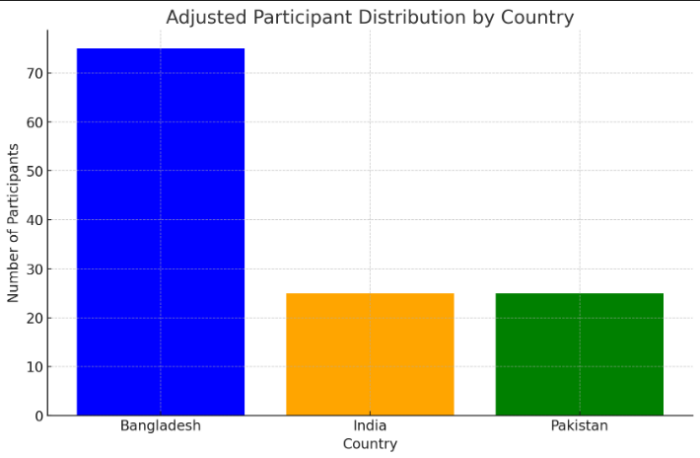
\includegraphics[width=0.8439\columnwidth,trim=0.0000bp 0.0000bp 0.0000bp 0.0000bp,clip]{figures/original_01.png}
\caption{Country distribution in the reported survey (n = 125). ``Adjusted'' is retained from the original graphic; no adjustment or weighting procedure is documented.}
\label{fig:f1}
\end{inlinefigure}


\begin{inlinefigure}
\centering
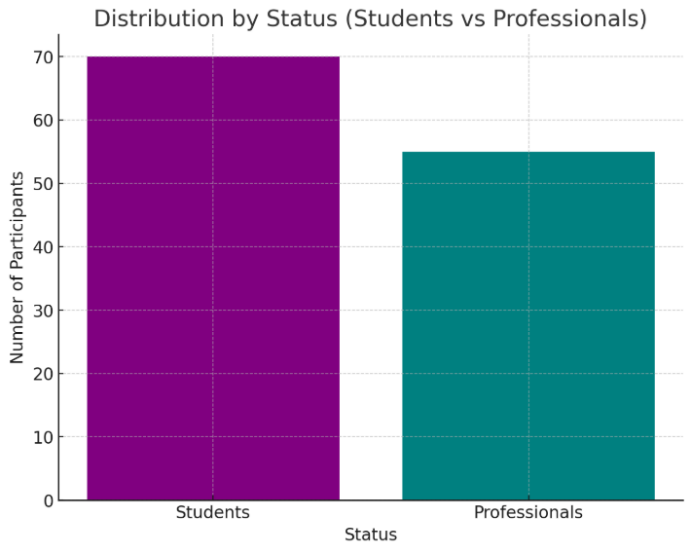
\includegraphics[width=0.8427\columnwidth,trim=0.3273bp 1.6364bp 0.0000bp 0.0000bp,clip]{figures/original_02.png}
\caption{Student and professional composition of the reported survey (n = 125). Original survey graphic.}
\label{fig:f2}
\end{inlinefigure}


Environmental science and civil engineering contribute 50 and 45 participants, respectively, together representing 76.0\% of the sample. Mechanical engineering contributes 10 (8.0\%), computer science engineering 12 (9.6\%), and electrical and electronic engineering 8 (6.4\%). Fig.~\ref{fig:f3} shows these proportions. The five discipline counts are 8, 10, 12, 45, and 50 when ordered; their median is 12. Fig.~\ref{fig:f4} summarizes the spread of those five aggregate counts and should not be interpreted as a distribution of participant-level responses.

\begin{inlinefigure}
\centering
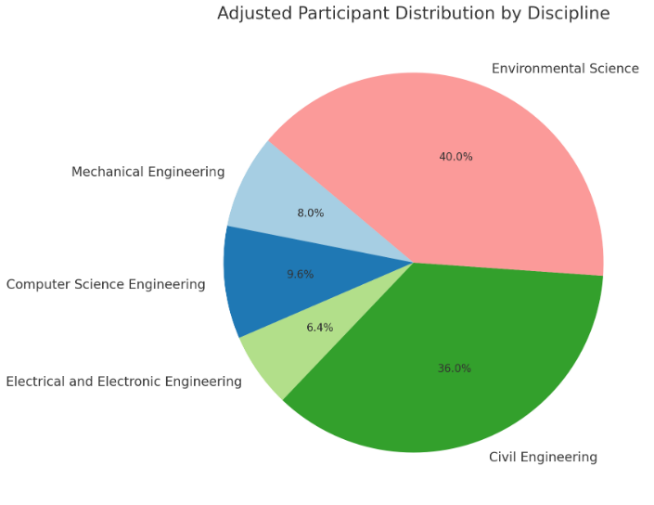
\includegraphics[width=0.8349\columnwidth,trim=0.0000bp 10.4732bp 2.2910bp 0.0000bp,clip]{figures/original_03.png}
\caption{Disciplinary composition (n = 125). Original graphic retained; ``Adjusted'' has no documented analytical definition.}
\label{fig:f3}
\end{inlinefigure}


\begin{inlinefigure}
\centering
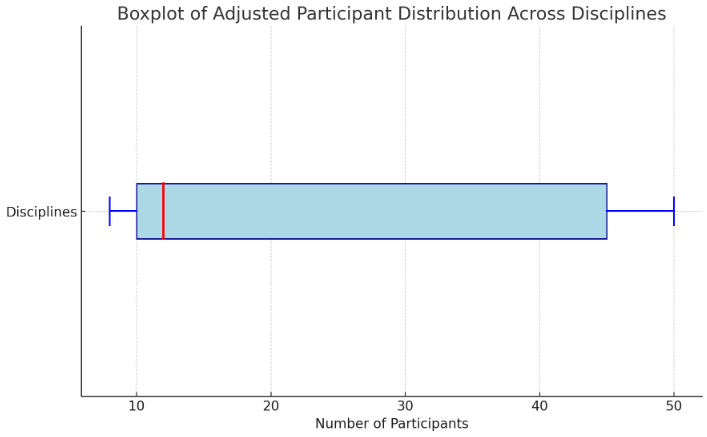
\includegraphics[width=0.9409\columnwidth,trim=0.0000bp 0.0000bp 0.0000bp 0.0000bp,clip]{figures/original_04.png}
\caption{Boxplot of the five discipline totals. The median count is 12; the plot does not describe an individual-level outcome.}
\label{fig:f4}
\end{inlinefigure}


\subsection{Perceptions of the concept}

The original summary image is retained in Fig.~\ref{fig:f5} as part of the study record. Experience or interest in flood management or water purification is reported by 57.6\%, with 42.4\% selecting ``No'' (Fig.~\ref{fig:f6}). Because experience and interest were grouped, the affirmative proportion must not be read as the proportion with practical expertise.

For technical feasibility, 44.8\% selected ``somewhat feasible'' and 39.2\% ``very feasible,'' giving 84.0\% favorable responses (Fig.~\ref{fig:f7}). Anticipated effectiveness received 48.8\% ``very effective'' and 37.6\% ``somewhat effective,'' totaling 86.4\% (Fig.~\ref{fig:f8}). Monitoring was considered ``very beneficial'' by 61.6\% and ``somewhat beneficial'' by 30.4\%, totaling 92.0\% (Fig.~\ref{fig:f9}). These ratings express expectations about the proposed system; they do not measure removal efficiency, dose delivery, or safety.

\begin{inlinefigure}
\centering
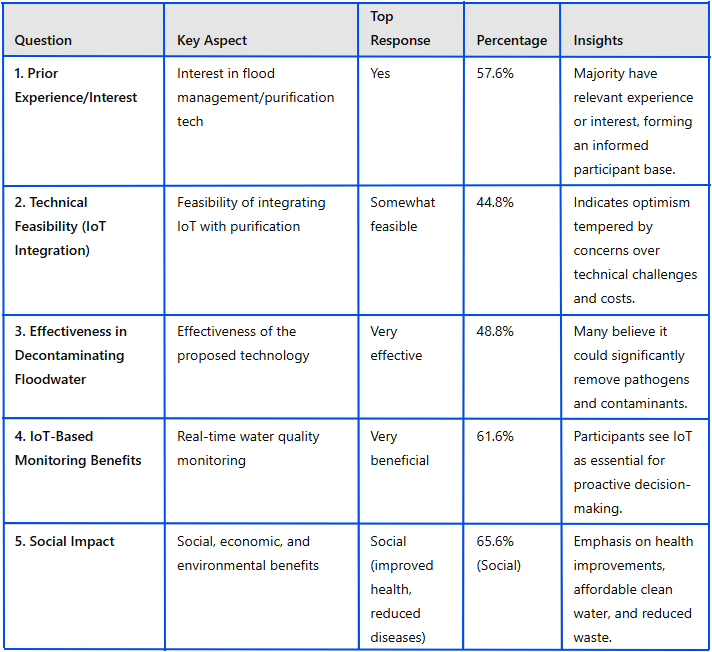
\includegraphics[width=0.97\columnwidth,trim=0.0000bp 0.0000bp 0.0000bp 0.0000bp,clip]{figures/original_05.png}
\caption{Original survey summary image. Its social-impact percentage conflicts with Fig.~\ref{fig:f10}; that entry is not used for substantive interpretation.}
\label{fig:f5}
\end{inlinefigure}


\begin{inlinefigure}
\centering
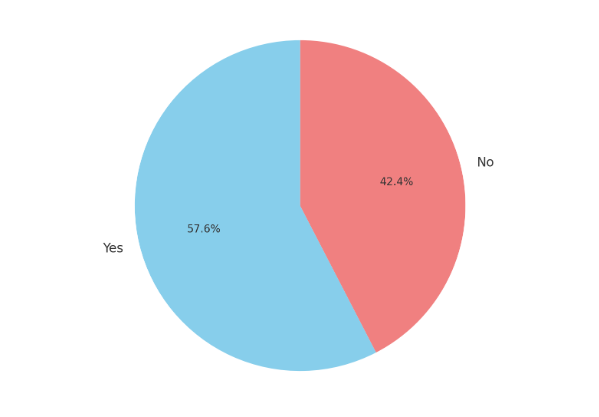
\includegraphics[width=0.5734\columnwidth,trim=71.2599bp 28.5040bp 72.7602bp 24.0034bp,clip]{figures/original_06.png}
\caption{Reported prior experience or interest in flood management or water purification (n = 125). Original survey graphic.}
\label{fig:f6}
\end{inlinefigure}




The impact item contains an unresolved numerical conflict. The narrative and summary image report social, environmental, and economic percentages of 65.6\%, 21.6\%, and 12.8\%, whereas the corresponding pie chart shows 36.6\%, 33.0\%, and 30.4\% (Fig.~\ref{fig:f10}). The underlying response records and denominator definitions are needed to reconcile these values. No quantified conclusion about the relative impact domains is drawn from this item.

\begin{inlinefigure}
\centering
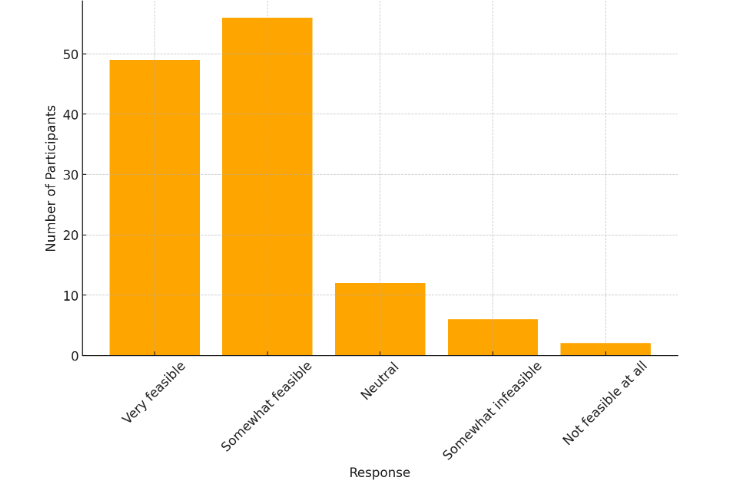
\includegraphics[width=0.8167\columnwidth,trim=27.0038bp 0.0000bp 47.2566bp 0.0000bp,clip]{figures/original_07.png}
\caption{Perceived technical feasibility of integrating IoT with UV-C and graphene-based treatment. Original survey graphic.}
\label{fig:f7}
\end{inlinefigure}


\begin{inlinefigure}
\centering
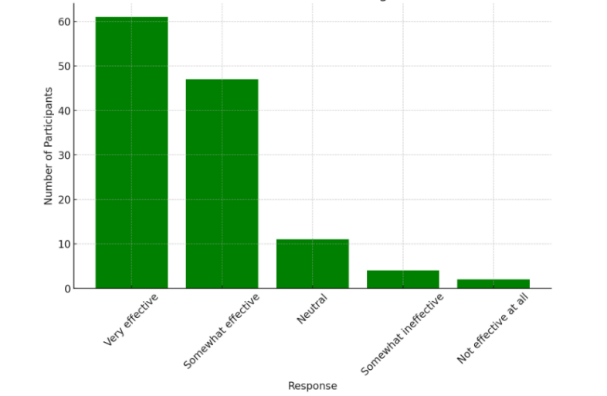
\includegraphics[width=0.8138\columnwidth,trim=11.4551bp 0.0000bp 15.3826bp 0.0000bp,clip]{figures/original_08.png}
\caption{Anticipated floodwater-decontamination effectiveness. The bars represent perceptions, not experimental removal percentages.}
\label{fig:f8}
\end{inlinefigure}


\begin{inlinefigure}
\centering
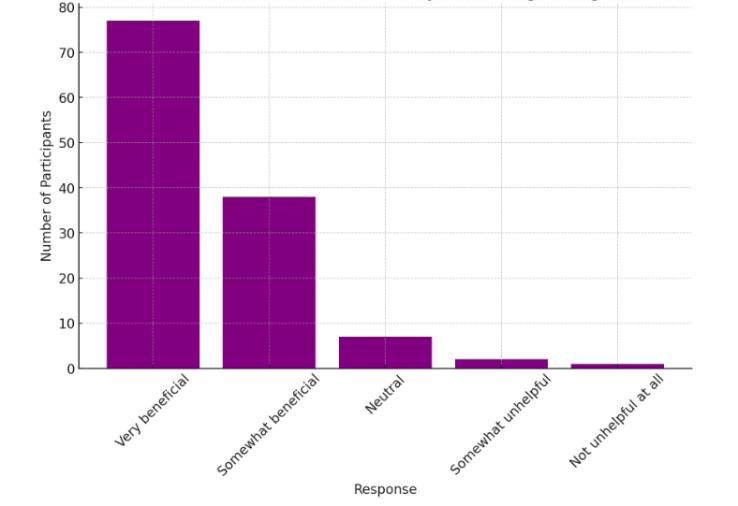
\includegraphics[width=0.8542\columnwidth,trim=10.1459bp 0.0000bp 12.1097bp 0.0000bp,clip]{figures/original_09.png}
\caption{Perceived benefit of real-time water-quality monitoring. Original survey graphic.}
\label{fig:f9}
\end{inlinefigure}




\begin{inlinefigure}
\centering
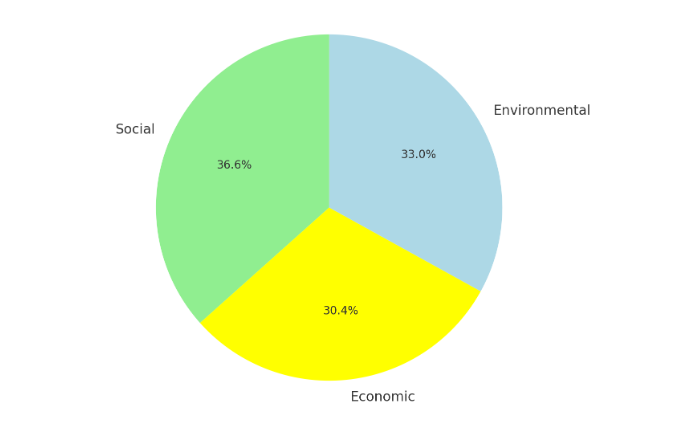
\includegraphics[width=0.6063\columnwidth,trim=81.0113bp 9.7514bp 63.0088bp 19.5027bp,clip]{figures/original_10.png}
\caption{Original impact pie chart, retained unchanged. Its displayed percentages conflict with the narrative and summary image; this item is excluded from interpretation pending reconciliation.}
\label{fig:f10}
\end{inlinefigure}


\subsection{Reported implementation concerns}



Among the 25 professionals in the reported interview component, 20 identified environmental conditions and 15 identified energy efficiency or scalability as concerns (Fig.~\ref{fig:f11}).

\begin{inlinefigure}
\centering
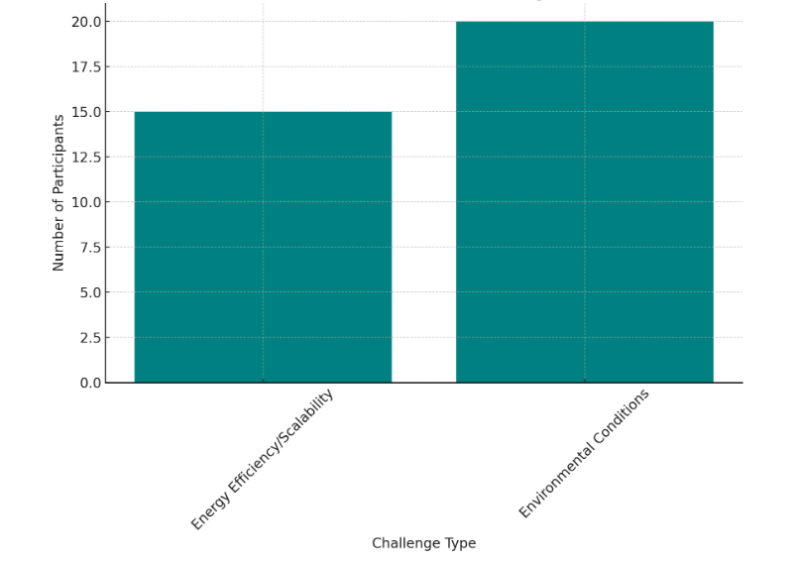
\includegraphics[width=0.8339\columnwidth,trim=14.0734bp 0.6546bp 15.7098bp 0.0000bp,clip]{figures/original_11.png}
\caption{Reported technical concerns in the 25-professional component. Categories may overlap; original graphic.}
\label{fig:f11}
\end{inlinefigure}


Affordability concerns were reported for 18 participants, while public-health benefits received combined agreement from 22 (Fig.~\ref{fig:f12}).

\begin{inlinefigure}
\centering
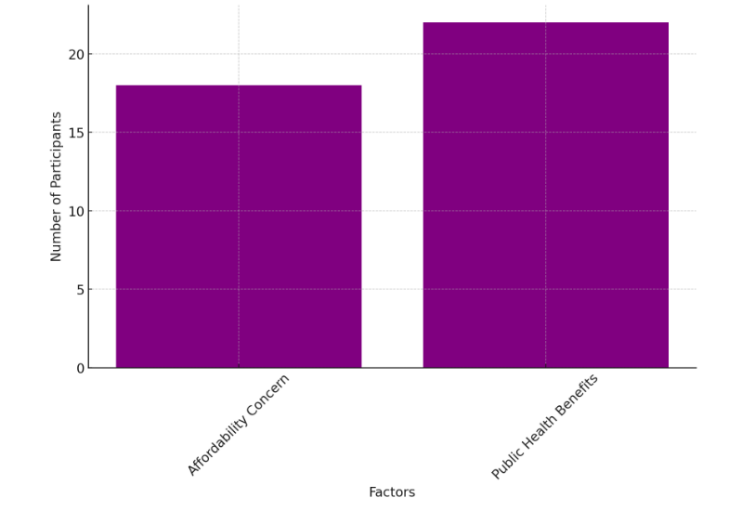
\includegraphics[width=0.8433\columnwidth,trim=13.4188bp 1.9637bp 11.7824bp 0.0000bp,clip]{figures/original_12.png}
\caption{Reported affordability concerns and agreement with anticipated public-health benefits (subsample n = 25). Original graphic.}
\label{fig:f12}
\end{inlinefigure}


Regional factors received agreement from 23, and cross-border relevance from 22 (Fig.~\ref{fig:f13}). These counts concern different prompts or categories and are not mutually exclusive shares of a single total. They indicate reported priorities without establishing the prevalence or independent coding of qualitative themes.

\begin{inlinefigure}
\centering
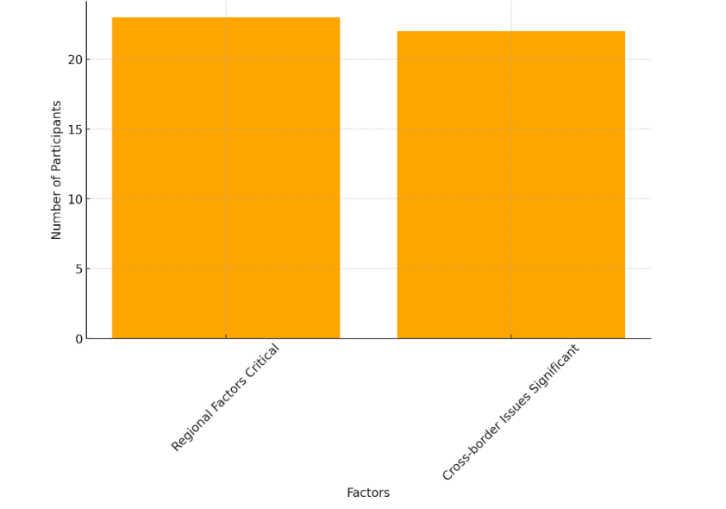
\includegraphics[width=0.8009\columnwidth,trim=13.7461bp 1.3092bp 21.6010bp 0.0000bp,clip]{figures/original_13.png}
\caption{Reported agreement with regional and cross-border considerations (subsample n = 25). Original graphic.}
\label{fig:f13}
\end{inlinefigure}


\subsection{Reproducible aggregate checks}

The demographic totals reconcile to 125, and the three combined favorable percentages reconcile arithmetically. Under a common denominator of 125, these percentages correspond to 105 favorable feasibility responses, 108 favorable effectiveness responses, and 115 favorable monitoring responses. These are reconstructed equivalents, not a replacement for an item-level response export. Fig.~\ref{fig:f14} records the calculation visually. The impact-item conflict remains unresolved; statistical software cannot determine which version is correct without the underlying records.

\begin{inlinefigure}
\centering
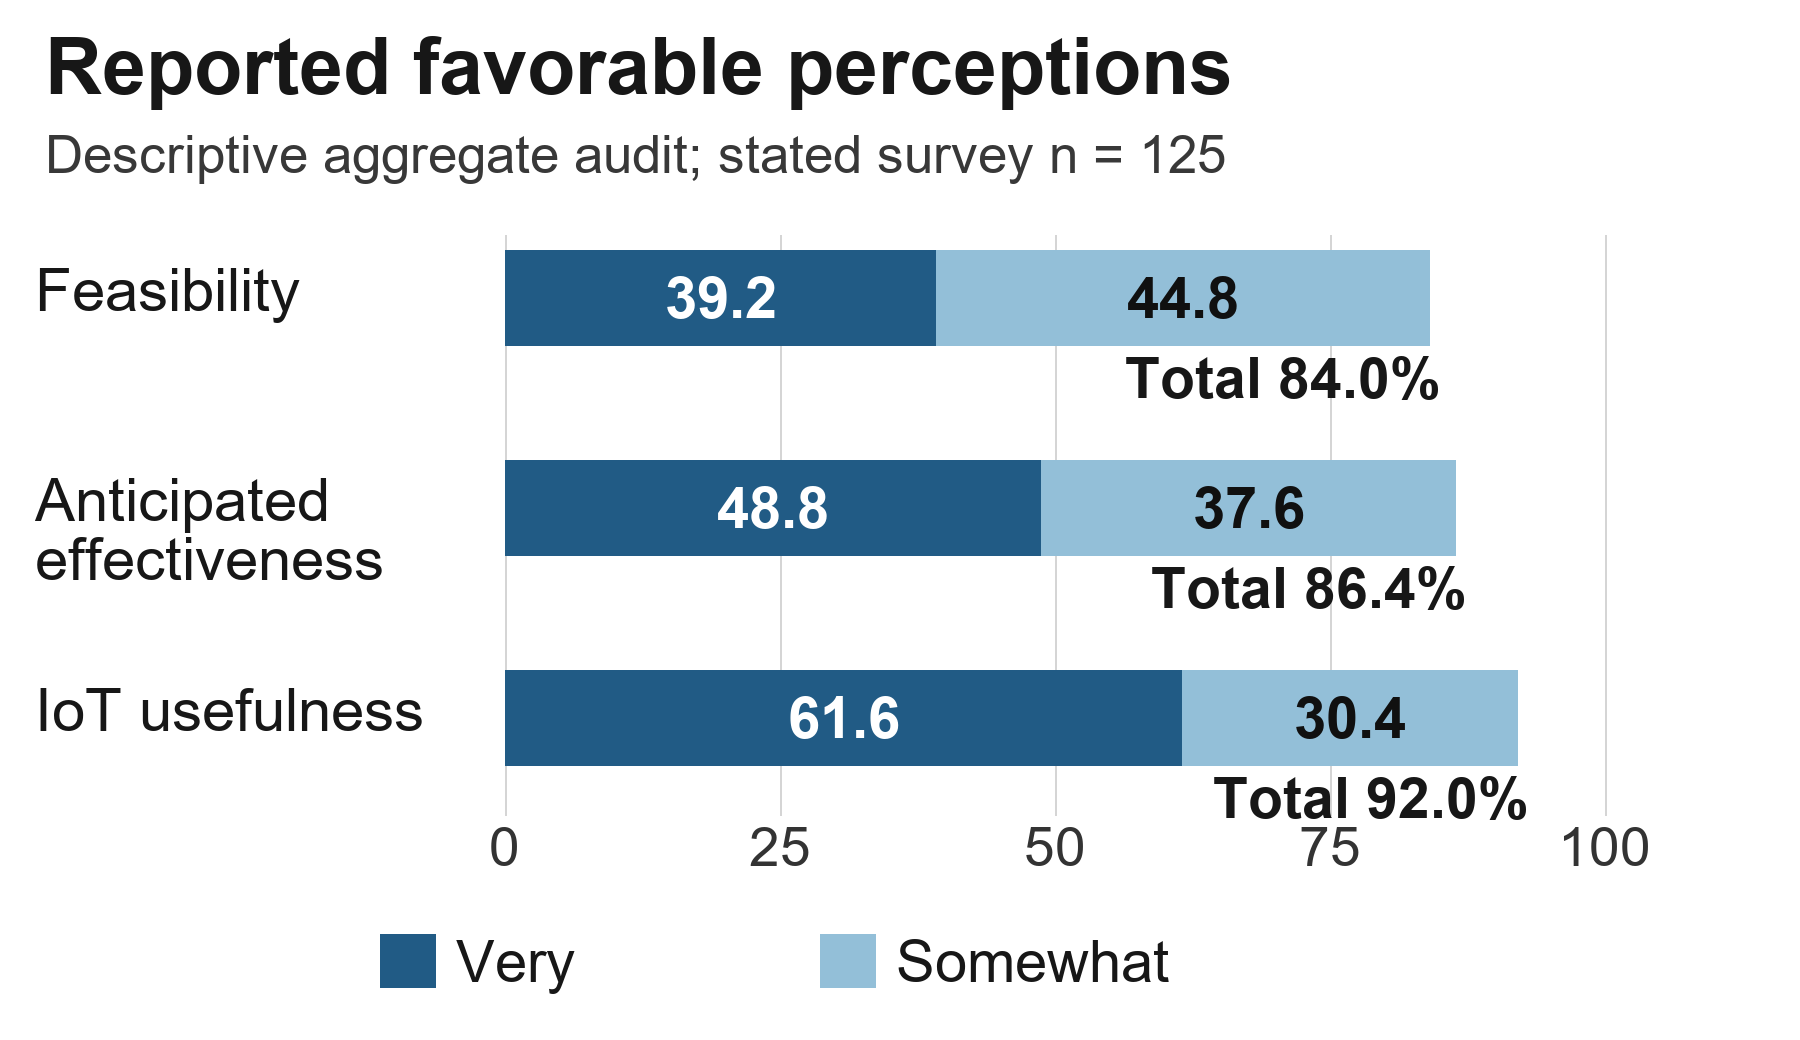
\includegraphics[width=0.8515\columnwidth,trim=3.2400bp 4.5600bp 17.2800bp 3.3600bp,clip]{figures/original_14.png}
\caption{Python arithmetic audit of the three reported perception items. Favorable totals combine the reported ``very'' and ``somewhat'' categories; bars are descriptive aggregates without inferential uncertainty intervals.}
\label{fig:f14}
\end{inlinefigure}


\section{Blueshield Filter Concept}

\subsection{Treatment sequence and pretreatment}

The proposed treatment train is intake screening, coagulation and flocculation, settling with sludge removal, a pressure-compatible supported GO-based cartridge, terminal UV-C disinfection, and protected storage. This ordering is an engineering interpretation of the component evidence \cite{r4,r5,r6,r7,r8,r9,r10,r11,r12}. The original component drawings are retained, while the revised sequence places the final disinfection barrier after filtration. Treatment modules require accessible sampling points so that each stage's contribution can be measured independently.

In the coagulation module (Fig.~\ref{fig:f15}), alum is a candidate coagulant. The dose and mixing conditions must be established by jar tests using representative source waters, with measurement of pH, alkalinity, clarified-water turbidity, and residual aluminium \cite{r4}, \cite{r5}. Coagulation destabilizes colloidal particles; flocculation promotes growth of aggregates, which settling or another solids-separation step removes. A universal 10--20 mg/L dose and a fixed motor speed are not established design specifications. Sludge removal and cleaning access are necessary design provisions.

\begin{inlinefigure}
\centering
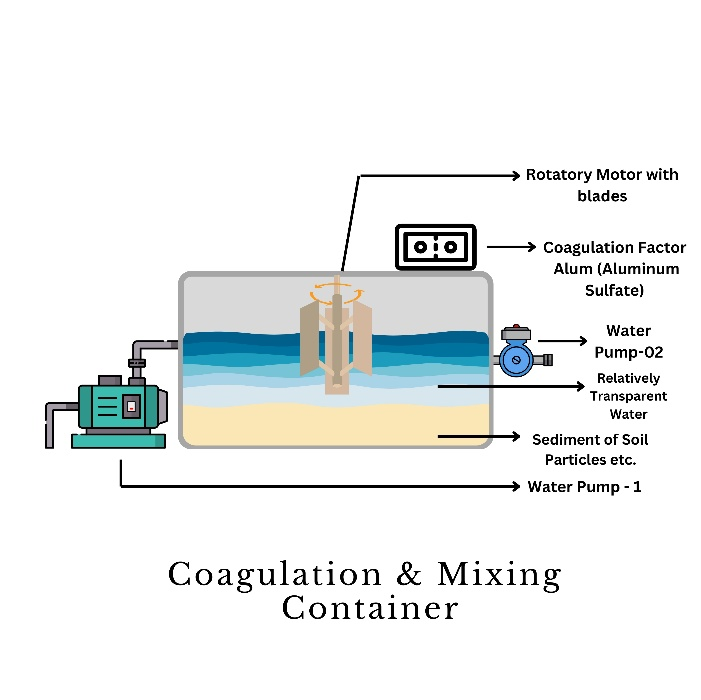
\includegraphics[width=0.8832\columnwidth,trim=12.1091bp 23.8909bp 1.9636bp 52.3636bp,clip]{figures/original_15.jpeg}
\caption{Authors' original Canva drawing of coagulation and mixing, retained unchanged. Equipment dimensions and operating settings remain unvalidated.}
\label{fig:f15}
\end{inlinefigure}

Figure~\ref{fig:coag_evidence} supplies an external example of why chemical residuals belong in the pretreatment assessment. Krupi\'nska compared four coagulants using a groundwater--surface-water mixture, with raw-water turbidity 10.6--15.0 NTU and pH 7.60--7.84~\cite{r5}. The residual-aluminium pattern varied with coagulant and dose. These conditions do not represent a validated BLUESHIELD floodwater envelope. In particular, the source dose is expressed as elemental Al per litre, whereas the illustrative mass accounting in Section~\ref{sec:engineering} uses commercial product mass. The results motivate measuring both clarification and aluminium residuals during jar tests; they do not select a universal coagulant or operating dose.

\begin{inlinefigure}
\centering
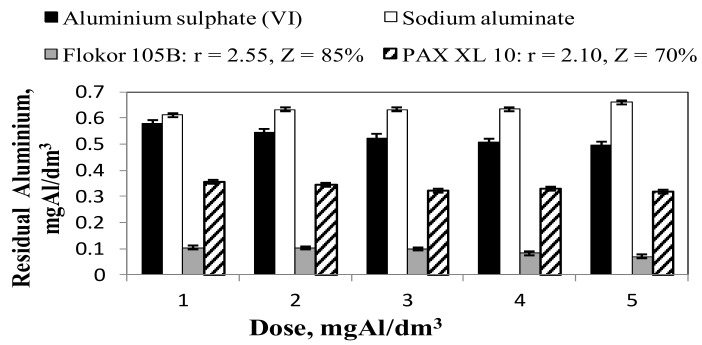
\includegraphics[width=0.98\columnwidth]{figures/krupinska2020_fig3.jpg}
\caption{External residual-aluminium results versus coagulant dose. The dose axis is mg Al/dm$^3$ (equivalent to mg Al/L), not mg/L commercial product. Source results are means of three jar tests; the plotted error-bar definition is not stated. $r$ and $Z$ describe coagulant alkalinity ratio and alkalinity percentage. Reproduced unchanged from Krupi\'nska~\cite{r5}, Fig.~3, \copyright\ 2020 the author, CC BY 4.0, \url{https://creativecommons.org/licenses/by/4.0/}. These are external experiments, not BLUESHIELD measurements.}
\label{fig:coag_evidence}
\end{inlinefigure}





\subsection{Defined graphene-based separation stage}

The graphene stage is specified as an immobilized GO composite on a suitable support, rather than loose nanosheets dispersed into product water. Fig.~\ref{fig:f16} preserves the original vessel concept. Membrane formulation, effective area, thickness, support, pore or interlayer structure, and operating pressure must be selected before flux and selectivity can be evaluated \cite{r6,r7,r8,r9}. A sorbent cartridge would require separate capacity and breakthrough measurements; adsorption and membrane rejection should not be treated as the same mechanism. Fig.~\ref{fig:f17} provides a spatial illustration of the vessel.

\begin{inlinefigure}
\centering
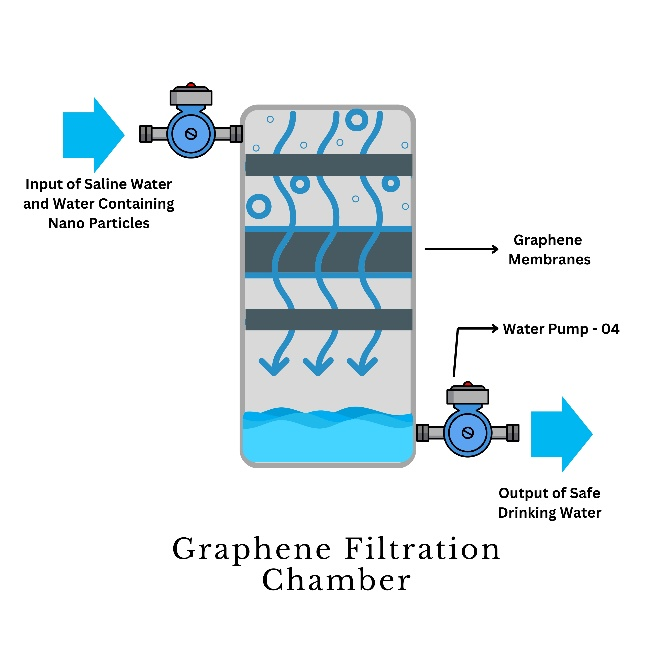
\includegraphics[width=0.8739\columnwidth,trim=4.9091bp 19.9636bp 10.4727bp 24.2182bp,clip]{figures/original_16.jpeg}
\caption{Authors' original Canva drawing of graphene filtration, retained unchanged. The original labels specify a proposed saline feed and intended drinking-water product; neither potability nor desalination has been demonstrated.}
\label{fig:f16}
\end{inlinefigure}


\begin{inlinefigure}
\centering
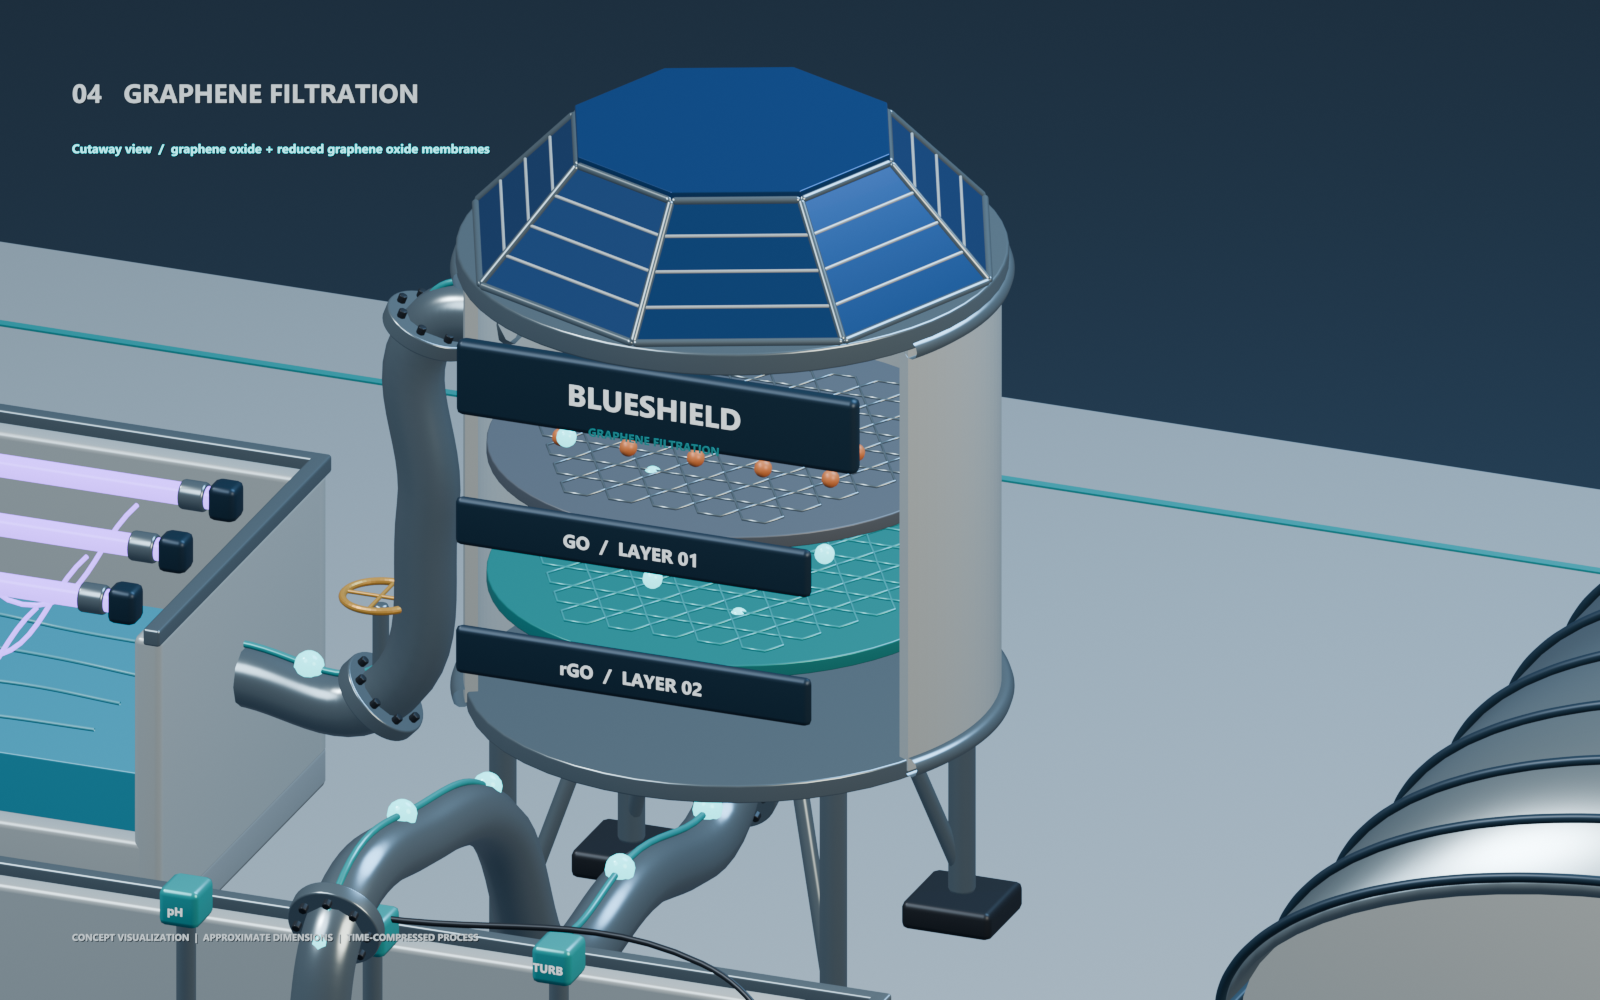
\includegraphics[width=0.9409\columnwidth,trim=0.0000bp 0.0000bp 0.0000bp 0.0000bp,clip]{figures/original_17.png}
\caption{Earlier Blender vessel cutaway retained from the project design. Layer arrangement and flow markers are illustrative. The revised integrated design places terminal UV-C after the supported membrane; no transport simulation or validated performance is represented.}
\label{fig:f17}
\end{inlinefigure}


Its GO and reduced-GO layers visualize candidate arrangements; they do not establish a fabricated membrane composition. Wet-state integrity, swelling, sealing, fouling, and release of carbonaceous material must be examined under the anticipated operating conditions \cite{r6}, \cite{r7}. Challenge testing should distinguish particulate removal, dissolved-solute rejection, and adsorptive uptake instead of reporting a single ``purification efficiency.''

\begin{inlinefigure}
\centering
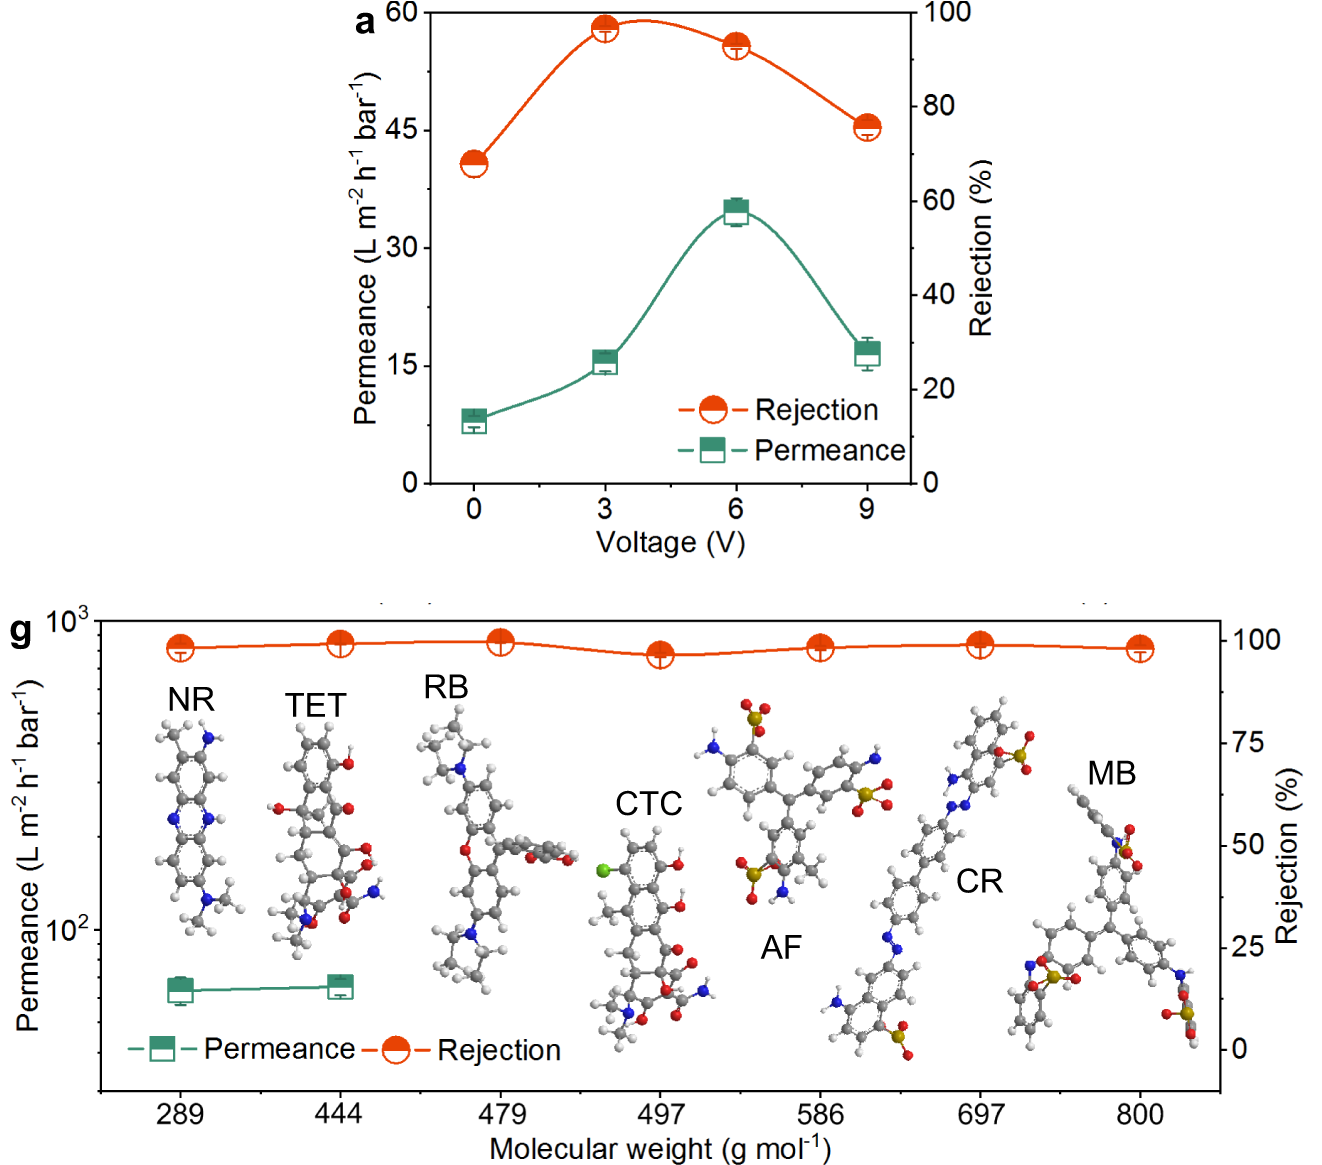
\includegraphics[width=0.9316\columnwidth,trim=0.4800bp 0.0000bp 2.6400bp 0.0000bp,clip]{figures/original_18.png}
\caption{External GO results at 2 bar: source Fig. 5(a), 200 \ensuremath{\mu}g membranes; Fig. 5(g), 50 \ensuremath{\mu}g PGO-6 membrane. PGO denotes porous GO; the suffix in PGO-3, PGO-6 and PGO-9 denotes a fabrication voltage of 3, 6 and 9 V, respectively. Error bars are standard deviations across three membranes. NR, TET, RB, CTC, AF, CR, and MB denote neutral red, tetracycline, rhodamine B, chlortetracycline hydrochloride, acid fuchsin, Congo red, and methyl blue. Reproduced from Liu et al. \cite{r9}, \textcopyright{} The Author(s) 2024, CC BY 4.0 (\url{https://creativecommons.org/licenses/by/4.0/}). Panels excerpted and stacked; data unchanged. These are not BLUESHIELD results.}
\label{fig:f18}
\end{inlinefigure}


Published separation results illustrate the need for this specificity. In the porous-GO study by Liu et al., sodium-sulfate separation depended on membrane preparation and test conditions, while sodium-chloride rejection was substantially lower \cite{r9}. Fig.~\ref{fig:f18} reproduces selected experimental panels as external material evidence. These data support testing an engineered separation layer; they cannot be transferred as BLUESHIELD removal rates or as proof of saline-floodwater desalination.

Recent membrane research continues to support architecture-specific evaluation. Han et al. demonstrated that arranging modified GO flakes within an asymmetric porous support altered ion-sieving performance and stability \cite{r17}. This provides a further candidate design principle, but its tested metal-salt separations and laboratory operating conditions do not establish general floodwater performance. BLUESHIELD requires its own material characterization and challenge tests before selecting such an architecture.

\subsection{Terminal UV-C disinfection}

The UV-C chamber (Fig.~\ref{fig:f19}) is a terminal treatment barrier whose performance must be linked to delivered fluence, wavelength, flow distribution, and water UV transmittance \cite{r10,r11,r12}. The original 6 W lamp label is a nominal component rating. It cannot establish a germicidal dose or a microbial log reduction.

\begin{inlinefigure}
\centering
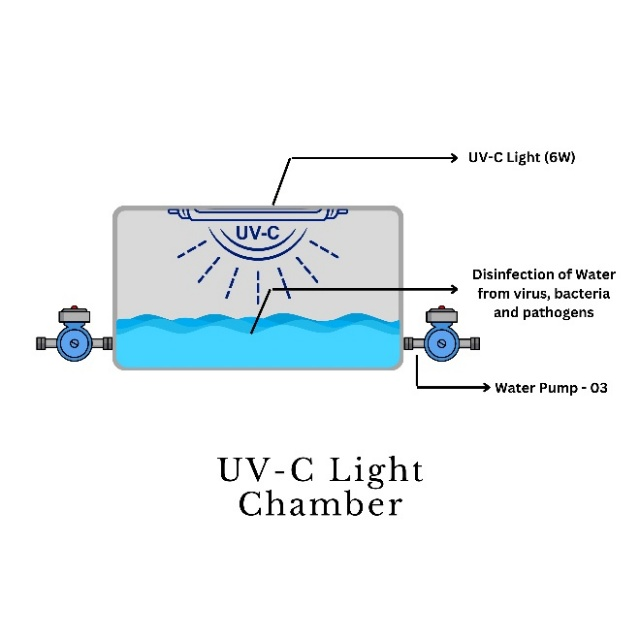
\includegraphics[width=0.8777\columnwidth,trim=8.8364bp 37.9636bp 5.2364bp 46.8000bp,clip]{figures/original_19.jpeg}
\caption{Authors' original Canva UV-C drawing, retained unchanged with its original 6 W label. Electrical wattage does not establish delivered fluence or disinfection performance.}
\label{fig:f19}
\end{inlinefigure}


For an idealized uniform field, fluence equals in-water fluence rate multiplied by exposure time. Real reactors require validation that accounts for the least-exposed flow paths, lamp ageing, sleeve fouling, and variation in feed-water transmittance. Particle-associated shielding is a further reason to clarify water before UV \cite{r11}. The external dose-response evidence in Fig.~\ref{fig:f20} illustrates the type of reactor evaluation required \cite{r12}. A proposed fail-closed outlet should prevent dispensing during lamp failure, excessive flow, or operation outside a validated treatment envelope. Setpoints remain to be established experimentally.

\begin{inlinefigure}
\centering
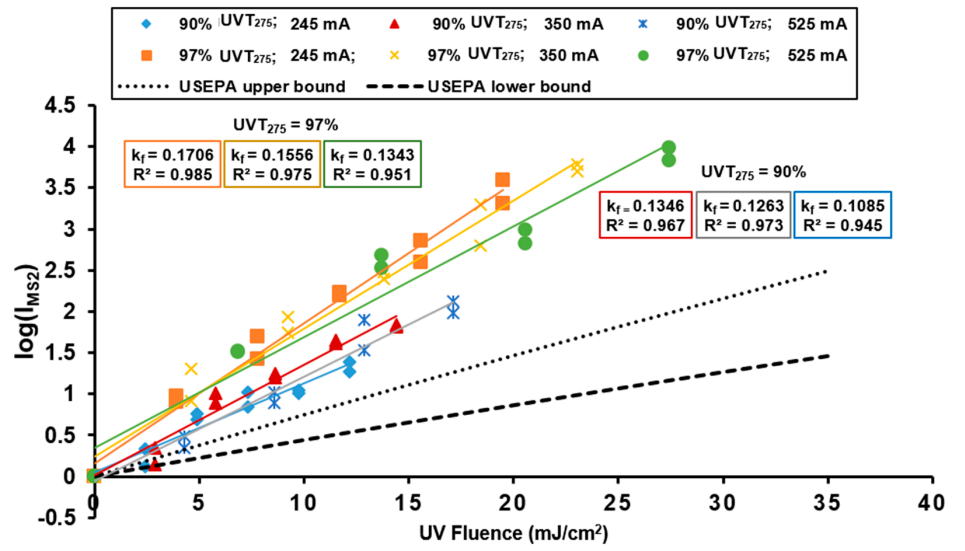
\includegraphics[width=0.9233\columnwidth,trim=2.0000bp 0.0000bp 4.0000bp 0.0000bp,clip]{figures/original_20.png}
\caption{External bench-scale UV-LED dose-response for MS2 bacteriophage, compared with mercury-UV reference curves. UVT$_{275}$ denotes UV transmittance at 275 nm. From Jarvis et al. \cite{r12}, Fig. 4. Reproduced \textcopyright{} The Authors 2019 under CC BY 4.0 (\url{https://creativecommons.org/licenses/by/4.0/}), without changing the plotted results. Source-specific MS2 challenge results do not validate BLUESHIELD.}
\label{fig:f20}
\end{inlinefigure}


\subsection{Monitoring and protected storage}

The proposed sensor package measures pH, temperature, turbidity, and conductivity-derived TDS, with flow and UV status included for process supervision. Calibration against reference instruments, drift checks, cleaning, and local data retention are required because low-cost measurements are sensitive to deployment conditions \cite{r13}, \cite{r14}. The controller should provide local alarms and retain essential functions during loss of connectivity. A dashboard can communicate operating status; it cannot certify microbial or chemical safety from these indicators alone.

Treated water should enter a protected vessel with hygienic dispensing, controlled access, and a documented cleaning procedure. Storage performance and water quality at the point of use require evaluation, as demonstrated by household field research \cite{r2}, \cite{r3}. Where source-water salinity or a dissolved contaminant exceeds the demonstrated capability of the selected cartridge, the design requires a separately validated treatment option or an alternative water source. Power demand, throughput, consumable life, and cost per treated volume remain evaluation outcomes, not established attributes of the concept.



\subsection{Three-dimensional stage visualization}
The authors' Canva drawings retain the original design record. New Blender geometries with flat two-dimensional annotations in Figs.~\ref{fig:stages12}--\ref{fig:stages56} make the proposed interfaces and maintenance provisions explicit. The models are explanatory, not dimensioned fabrication drawings, manufactured prototypes or fluid/optical simulations. Blue process paths, separate residuals handling, supported media and an enclosed UV chamber express design intent. Dimensions, materials and operating setpoints require subsequent engineering verification.

Screening and access for debris removal precede rapid mixing and gentle flocculation (Fig.~\ref{fig:stages12}). Settling requires a decant outlet separated from accumulated sludge; carrying flocs directly into the GO cartridge would undermine its pretreatment role. The separation models in Fig.~\ref{fig:stages34} depict settling and supported, immobilized membrane media with an inlet, permeate outlet, pressure observation and residuals handling. The GO arrangement does not assert a particular commercial membrane formulation. The terminal-stage models in Fig.~\ref{fig:stages56} place UV treatment after the membrane in a closed chamber with provision for sleeve access and flow supervision. Protected storage and hygienic dispensing complete the train, while local sensing supports operational decisions.
\end{multicols}
\begin{inlinefigure}
\centering
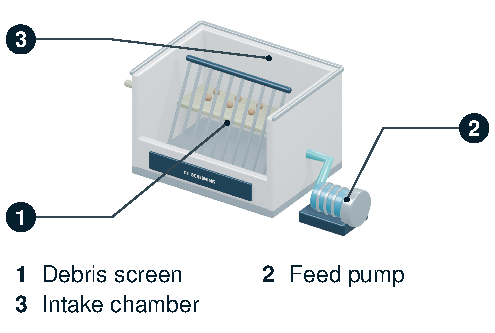
\includegraphics[width=0.48\textwidth]{figures/01_Intake_and_Screen.pdf}\hfill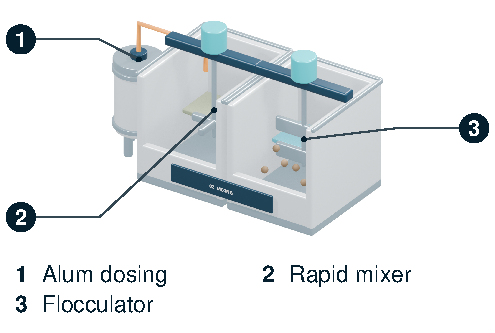
\includegraphics[width=0.48\textwidth]{figures/02_Coagulation_and_Flocculation.pdf}
\par\makebox[0.48\textwidth]{(a)}\hfill\makebox[0.48\textwidth]{(b)}
\caption{Proposed intake and pretreatment in Blender. (a) Screened intake with accessible debris removal. (b) Coagulant addition, rapid mixing and gentle flocculation. Rendered vessels and impellers are conceptual geometries; dose and mixing conditions require jar tests.}\label{fig:stages12}
\end{inlinefigure}

\begin{inlinefigure}
\centering
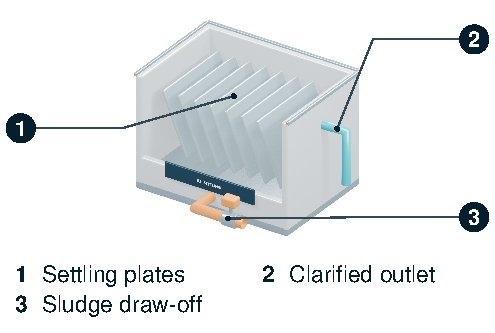
\includegraphics[width=0.48\textwidth]{figures/03_Settling_and_Sludge.pdf}\hfill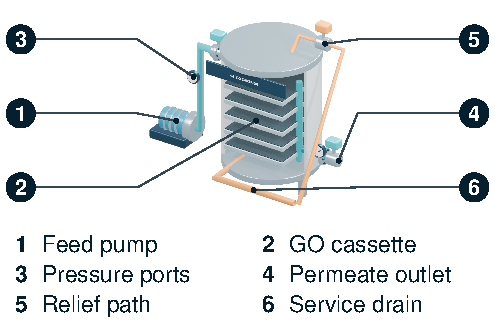
\includegraphics[width=0.48\textwidth]{figures/04_Supported_GO_Cartridge.pdf}
\par\makebox[0.48\textwidth]{(a)}\hfill\makebox[0.48\textwidth]{(b)}
\caption{Proposed separation stages in Blender. (a) Settling vessel with a distinct sludge withdrawal route. (b) Supported GO cartridge cutaway with contained media and pressure-loop provisions. The cutaway is a structural illustration, not a molecular-scale or pressure-vessel validation.}\label{fig:stages34}
\end{inlinefigure}

\begin{inlinefigure}
\centering
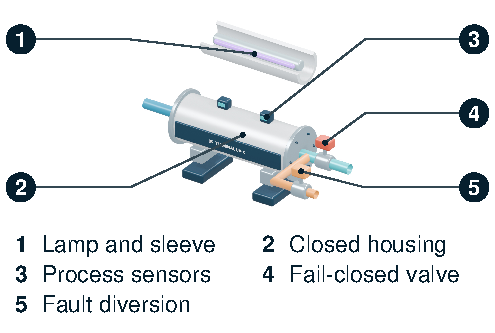
\includegraphics[width=0.48\textwidth]{figures/05_Terminal_UVC_Reactor.pdf}\hfill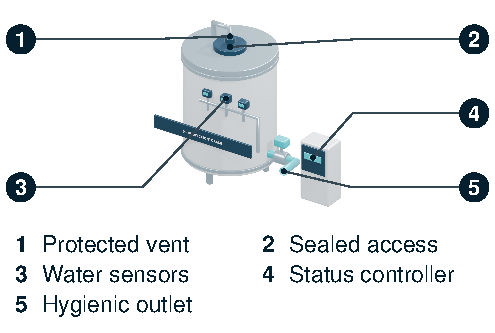
\includegraphics[width=0.48\textwidth]{figures/06_Protected_Storage_and_Sensing.pdf}
\par\makebox[0.48\textwidth]{(a)}\hfill\makebox[0.48\textwidth]{(b)}
\caption{Proposed terminal barriers in Blender. (a) Enclosed UV-C reactor with an internal explanatory view. (b) Protected storage and monitoring. Final UV follows filtration; sensing and valve control require calibration and functional testing. No water-safety outcome is inferred from the render.}\label{fig:stages56}
\end{inlinefigure}
\begin{multicols}{2}


\section{Preliminary engineering assessment}
\label{sec:engineering}
The survey identifies perceived value and implementation concerns; it does not provide hydraulic or treatment parameters. The following calculations translate those concerns into testable design requirements. Every numerical input in Table~\ref{tab:assumptions} is an illustrative assumption selected for a small batch unit. None is estimated from respondent ratings or presented as a measured BLUESHIELD specification. These calculations are a screening assessment, without transport simulation, optimization, or experimental validation.

\begin{inlinetable}
\caption{Illustrative inputs and calculated quantities for a small batch unit. All inputs are assumptions; all outputs are conditional calculations.}
\label{tab:assumptions}
\centering\small
\begin{tabular}{p{0.52\columnwidth}p{0.38\columnwidth}}
\toprule
Quantity & Value and status\\
\midrule
Raw batch volume, $V_b$ & 20 L; assumed\\
Recoverable fraction, $f_r$ & 0.90; assumed\\
Flow during discharge, $Q_p$ & 10 L/h; assumed\\
Rapid mixing / flocculation & 1 / 20 min; assumed\\
Quiescent settling & 60 min; assumed\\
Product volume, $V_p$ & 18 L; calculated\\
Discharge time & 1.80 h; calculated\\
Cycle time & 3.15 h; calculated\\
Cycle-average output & 5.71 L/h; calculated\\
\bottomrule
\end{tabular}
\end{inlinetable}

\subsection{Batch throughput and coagulant accounting}
For sequential mixing, settling and discharge, the volume and time balances are
\begin{equation}
\begin{split}
V_p&=f_r V_b,\\
t_{\mathrm{cycle}}&=t_{\mathrm{rapid}}+t_{\mathrm{floc}}+t_{\mathrm{settle}}+V_p/Q_p,\\
\overline{Q}_p&=V_p/t_{\mathrm{cycle}}.
\end{split}
\label{eq:cycle}
\end{equation}
The example produces a calculated cycle-average output of 5.71 L/h, even though water is discharged at 10 L/h. Filling, cleaning and operator delays are omitted, so actual average delivery could be lower. The assumed 90\% recoverable fraction is a lumped allowance for volume loss; it does not establish membrane recovery, concentrate handling or sustainable operation. A plant with parallel tanks would require a separate scheduling and mass-balance model.

Alum addition can be accounted for without assuming a universally effective dose. For commercial-product dose $D$ in mg/L, batch volume $V_b$ in L and stock concentration $C_s$ in mg/L of the same product,
\begin{equation}
m_a=\frac{D V_b}{1000}\ [\mathrm{g}],\qquad
V_s=\frac{D V_b}{C_s}\ [\mathrm{L}].
\label{eq:alum}
\end{equation}
Illustrative doses of 10, 30 and 50 mg/L would require 0.20, 0.60 and 1.00 g per 20-L batch, respectively. These are accounting examples, not treatment recommendations. With an assumed 10\,000-mg/L stock, the corresponding additions are 20, 60 and 100 mL. Commercial grade, hydrate and assay must be specified because product mass and elemental-aluminium mass are different dose bases. Source-specific jar tests must establish the dose, mixing sequence and settling conditions~\cite{epa_turbidity2004}. Stock additions are neglected in the approximate cycle example and must be included in a final balance.

The bulk velocity-gradient relation is
\begin{equation}
G=\sqrt{\frac{P_w}{\mu V}},\qquad P_w=\mu V G^2,
\label{eq:mixing}
\end{equation}
where $G$ is in s$^{-1}$, $P_w$ is power dissipated into water in W, $\mu$ is viscosity in Pa\,s, and $V$ is water volume in m$^3$~\cite{epa_nutrient2010}. Assuming $\mu=10^{-3}$ Pa\,s and $V=0.020$ m$^3$, gradients of 700 and 50 s$^{-1}$ imply fluid powers of 9.8 and 0.050 W. Neither value specifies motor demand, impeller speed or local floc shear. Settling effectiveness must likewise be measured; a selected holding time cannot be converted directly to a turbidity-removal percentage.

\subsection{Membrane area and pressure compatibility}
For a defined supported membrane, operating flux $J$, apparent applied-pressure permeance $L_{p,\mathrm{app}}$ and solute rejection $R_i$ are
\begin{equation}
J=\frac{Q_p}{A_m},\quad
L_{p,\mathrm{app}}=\frac{J}{\Delta P},\quad
R_i=1-\frac{C_{p,i}}{C_{f,i}}.
\label{eq:membrane}
\end{equation}
Here $J$ is in L\,m$^{-2}$\,h$^{-1}$ (LMH), $A_m$ in m$^2$, and feed and permeate concentrations use matching units. $\Delta P$ is transmembrane pressure; for cross-flow, it is approximately $(P_f+P_r)/2-P_p$, using feed, retentate and permeate pressures. It is distinct from the total pump differential. These definitions are consistent with the controlled experiments in~\cite{r9}; their reported results are not input performance values for this design. $L_{p,\mathrm{app}}$ depends on the solution and operating conditions and is not a universal material constant. Salinity, osmotic effects and concentration polarization require further treatment before a desalination model is possible.

At the assumed $Q_p=10$ L/h, operating fluxes of 10, 25 and 50 LMH require 1.00, 0.40 and 0.20 m$^2$ of active membrane area. If a hypothetical 25-LMH operating condition falls by 50\% through fouling, a 0.40-m$^2$ cartridge would discharge only 5 L/h. Figure~\ref{fig:sensitivity} shows the sensitivity to active area and batch timing. The curve contains no fitted experimental parameters.

\end{multicols}
\begin{inlinefigure}
\centering
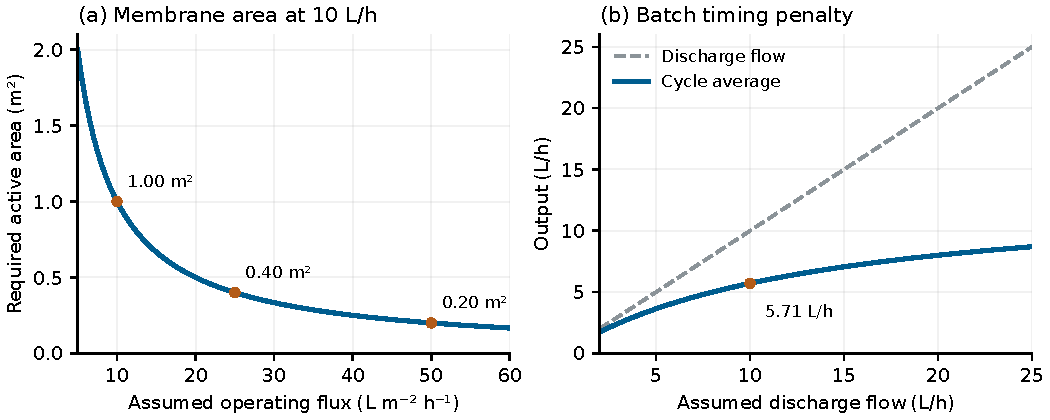
\includegraphics[width=0.98\textwidth]{figures/design_sensitivity.pdf}
\caption{Calculated design sensitivities. (a) Active area required for 10 L/h over assumed operating fluxes; the highlighted values are illustrative inputs. (b) Cycle-average output for an assumed 18-L recoverable batch and 81-min combined mixing and settling time, compared with instantaneous discharge flow. These are deterministic calculations, not BLUESHIELD test results; no empirical uncertainty intervals are available.}
\label{fig:sensitivity}
\end{inlinefigure}
\begin{multicols}{2}

The available pressure must be compatible with the membrane assumption. Hydrostatic head gives
\begin{equation}
\Delta P=\rho g h.
\label{eq:head}
\end{equation}
With rounded water density $\rho=1000$ kg/m$^3$, $g=9.81$ m/s$^2$ and $h=0.50$ m, the head is only 0.0491 bar. An explicitly hypothetical linear extrapolation of 25 LMH/bar would then yield 1.23 LMH and require approximately 8.15 m$^2$ to supply 10 L/h. This optimistic illustration neglects additional losses and is not a low-pressure membrane prediction. Conversely, 1 bar corresponds to approximately 10.2 m of water head. A compact gravity vessel therefore cannot inherit flux measured in a pressurized laboratory cell. A pumped concept needs a rated housing, seals, relief provision and a defined reject or cleaning route.

\subsection{UV exposure and pumping work}
For a microorganism following trajectory $j$, delivered fluence is the time integral of the in-water fluence rate~\cite{epa_uv2006}:
\begin{equation}
H_j=\int_0^{t_j} E_f(\mathbf{x}_j(t),t)\,\mathrm{d}t.
\label{eq:uvpath}
\end{equation}
An ideal uniform-field, plug-flow calculation gives
\begin{equation}
H_{\mathrm{nom}}=\overline{E}_f\frac{V_{\mathrm{UV}}}{Q},\qquad
V_{\mathrm{UV,ideal}}=\frac{Q H_{\mathrm{study}}}{\overline{E}_f}.
\label{eq:uvvolume}
\end{equation}
When fluence rate is mW/cm$^2$ and fluence is mJ/cm$^2$, time must be in seconds. Thus $Q$ in L/h is divided by 3600 before the volume calculation. Table~\ref{tab:uv} uses an assumed study fluence of 40 mJ/cm$^2$; this is a sensitivity target, not a universal safety threshold. The volume excludes the lamp sleeve and displaced solids. Real reactors exhibit distributions of exposure, and neither nominal residence time nor electrical wattage establishes a validated reduction-equivalent dose.

\begin{inlinetable}
\caption{Ideal UV sizing at assumed flow 10 L/h and study fluence 40 mJ/cm$^2$. Optical inputs are independent assumptions.}
\label{tab:uv}
\centering\small
\begin{tabular}{ccc}
\toprule
Fluence rate & Exposure & Water volume\\
(mW/cm$^2$) & (s) & (L)\\
\midrule
0.25 & 160 & 0.444\\
0.50 & 80 & 0.222\\
1.00 & 40 & 0.111\\
\bottomrule
\end{tabular}
\end{inlinetable}

The pump energy requirement follows a hydraulic work balance~\cite{doe_pump2005}:
\begin{equation}
P_{\mathrm{el}}=\frac{\Delta P_{\mathrm{tot}}Q_{\mathrm{pump}}}{\eta_{\mathrm{sys}}},\qquad
e_{\mathrm{pump}}=\frac{\Delta P_{\mathrm{tot}}}{3.6\times10^6\eta_{\mathrm{sys}}}.
\label{eq:energy}
\end{equation}
Pressure is in Pa, pump flow in m$^3$/s, power in W and specific energy in kWh per m$^3$ pumped. With assumed overall efficiency 0.30, total pressure differentials of 0.5 and 2.0 bar give 0.0463 and 0.1852 kWh/m$^3$ pumped. At 10 L/h, the corresponding calculated powers are 0.463 and 1.852 W. Miniature-pump losses, recirculation and the operating point may increase actual draw. These pressures do not imply equal membrane flux. Total treatment energy must additionally include measured mixing, UV, controls, standby and cleaning demand per delivered volume. No relationship is asserted between the original 6-W lamp label and the optical assumptions in Table~\ref{tab:uv}.

\subsection{Validation endpoints}
Removal claims require matched influent and effluent measurements. For the same viable or infective organism and assay basis,
\begin{equation}
\mathrm{LRV}_i=\log_{10}\left(\frac{N_{\mathrm{in},i}}{N_{\mathrm{out},i}}\right),\qquad
\eta_i=1-10^{-\mathrm{LRV}_i}.
\label{eq:lrv}
\end{equation}
A nondetect is bounded by an assay detection limit; it is never entered as zero in the logarithm. Stage log reductions can only be combined using compatible consecutive measurements, not selected values from unrelated papers. All BLUESHIELD log-reduction values remain unmeasured. The WHO household-water-treatment testing protocol supplies a framework for prospective microbial challenges across organism classes and operating life~\cite{who_hwt2018}. The present concept has no assigned WHO performance classification.

The calculations identify unresolved design constraints: waiting time reduces delivery, membrane area depends strongly on usable flux and pressure, and UV efficacy depends on hydraulic and optical validation. These findings turn the survey's feasibility, energy and monitoring concerns into measurable prototype questions.


\section{Discussion}

The main perception items show support for evaluating BLUESHIELD, particularly its monitoring function. Their practical value lies in identifying what participants expect and which constraints deserve attention. Environmental conditions and energy concerns connect the survey to pretreatment, source-water characterization, and operating-envelope validation. Affordability concerns support evaluating recurring consumables, maintenance effort, and service availability alongside the purchase price. The survey does not quantify those costs or establish that the proposed system is affordable.

Table~\ref{tab:traceability} links the reported priorities to the proposed engineering response and to measurements needed in a later study. These links are the authors' design interpretation, not causal associations estimated from the survey. They provide a practical basis for testing the concept without treating favorable ratings as evidence of treatment capability.

\end{multicols}
\begin{inlinetable}
\caption{From reported survey priorities to prospective design evaluation. Percentages and counts retain the source limitations; design responses are proposed interpretations.}
\label{tab:traceability}\vspace{-6pt}
\centering\small
\renewcommand{\arraystretch}{1.00}
\begin{tabular}{p{0.265\textwidth}p{0.315\textwidth}p{0.34\textwidth}}
\toprule
Reported survey evidence & Proposed design response & Prospective measurement\\
\midrule
Feasibility favorable: 84.0\% & Modular stage interfaces and service access & Assembly, leakage, operator-task and maintainability tests\\
Anticipated effectiveness favorable: 86.4\% & Solids removal, supported membrane and terminal UV & Paired contaminant and microbial challenge measurements\\
Monitoring benefit favorable: 92.0\% & Local sensing, flow supervision and interlocks & Calibration error, drift and alarm/valve function under faults\\
Environmental conditions: 20 of 25 & Source-specific dosing and operating envelopes & Jar tests, UV transmittance, fouling and seasonal source variation\\
Energy or scalability: 15 of 25 & Explicit batch timing and pressure/flow accounting & Delivered volume and electrical energy over complete operating cycles\\
Affordability concern: 18 of 25 & Accessible consumables and service provision & Purchase, replacement, cleaning and service cost per delivered volume\\
\bottomrule
\end{tabular}\vspace{6pt}
\end{inlinetable}
\begin{multicols}{2}


The sample is concentrated in Bangladesh, students, civil engineering, and environmental science. Pooled ratings consequently reflect that composition, and no country or occupational comparison is justified without participant-level cross-tabulations and an appropriate sampling design. The reported interview counts add implementation priorities, but lack the transcripts, coding evidence, and participant quotations needed for a fully traceable qualitative interpretation. The impact-chart conflict further limits what can be concluded from that item.

Research on household treatment in Bangladesh provides a useful comparison. Luoto et al. show that assigned treatment, reported use, and stored-water microbial outcomes are distinct measurements \cite{r2}. The external results reproduced in Fig.~\ref{fig:f21} illustrate why favorable intentions should be followed by direct observation of use and water-quality measurement. Pickering et al. further support investigating user effort and service arrangements \cite{r3}. These findings motivate a future BLUESHIELD evaluation with flood-affected households and operators, rather than extending technical-stakeholder ratings to household adoption.

\begin{inlinefigure}
\centering
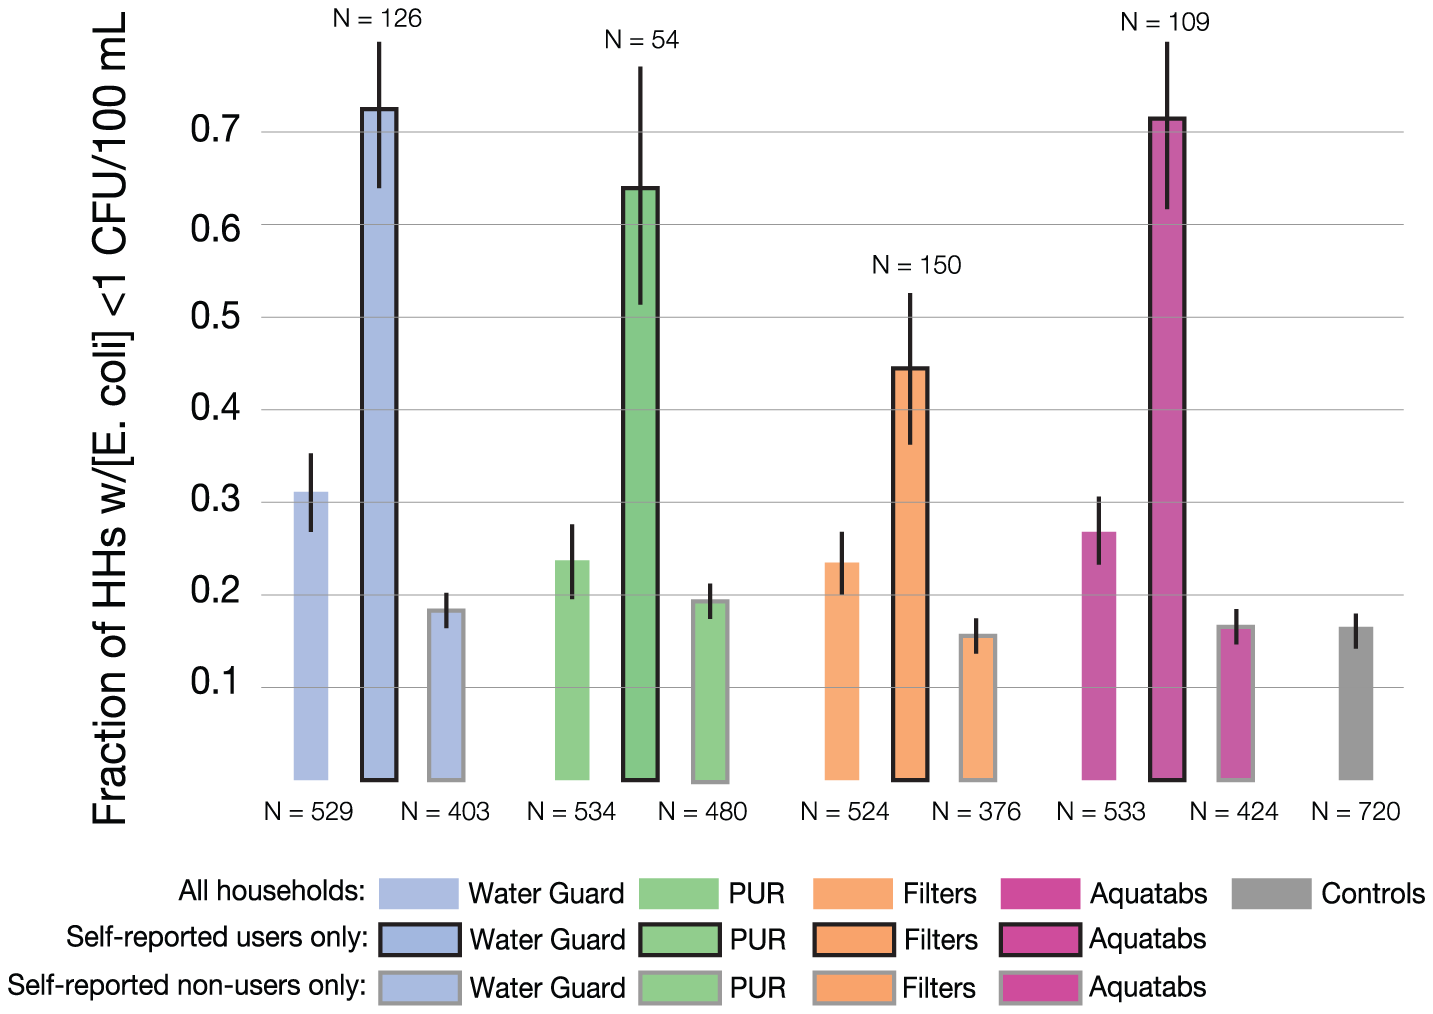
\includegraphics[width=0.9409\columnwidth,trim=0.0000bp 0.0000bp 0.0000bp 0.0000bp,clip]{figures/original_21.png}
\caption{External Bangladesh field evidence: stored water with no detectable E. coli, by assigned product and self-reported use during the previous 24 hours. Reproduced from Luoto et al. \cite{r2}, Fig. 2, \textcopyright{} 2011 Luoto et al., under the Creative Commons Attribution License stated in \cite{r2}. Error bars are source-study standard errors. Results concern the cited products, not BLUESHIELD.}
\label{fig:f21}
\end{inlinefigure}


The component evidence narrows the next engineering decisions. A defined GO architecture must demonstrate stable separation without unacceptable material release; the UV reactor must demonstrate microbial inactivation under realistic feed-water and flow conditions; and sensors must be verified as process instruments. An integrated prototype should then be evaluated through paired influent and effluent measurements, replicate operation, maintenance cycles, and storage testing. Comparisons with established treatment options are needed before claims about superiority, lower energy demand, environmental benefit, or health impact are warranted.

Seasonality also matters when planning the next survey. A longitudinal study of households in rural Bangladesh documented changes in water-insecurity experiences across the monsoon cycle \cite{r18}. A future BLUESHIELD study should therefore record recruitment season, local water sources, flood exposure, and household water responsibilities. These variables would allow the interpretation of user needs within their setting, provided that the survey instrument and sampling plan are specified before recruitment.

\subsection{Integrated machine and industrial installation}
The machine in Fig.~\ref{fig:machine} connects the stages in series, adds a GO feed-pressure loop and places UV-C after the membrane. Separate paths carry product, sludge and diverted water. An interlocked outlet is intended to close or divert flow during inadequate UV operation, excessive flow or other faults outside a validated envelope. Relief and diversion discharge require controlled holding, with no untreated bypass into product storage; pressure-relief settings require a rated mechanical design.

The industrial arrangement in Fig.~\ref{fig:industrial} develops the earlier setup with treatment modules, residuals handling and operator access. Scaling requires source-water characterization, continuous or staggered-batch mass balances, pipe and pump sizing, redundancy, cleaning access, electrical protection and waste management. Plant capacity and flood resilience require validation. Assessing the solar-panel option requires local irradiance data, battery sizing and measured electrical demand.

\end{multicols}
\par\vspace{2pt}\noindent\begin{minipage}{\linewidth}\makeatletter\def\@captype{figure}\makeatother\centering
\centering
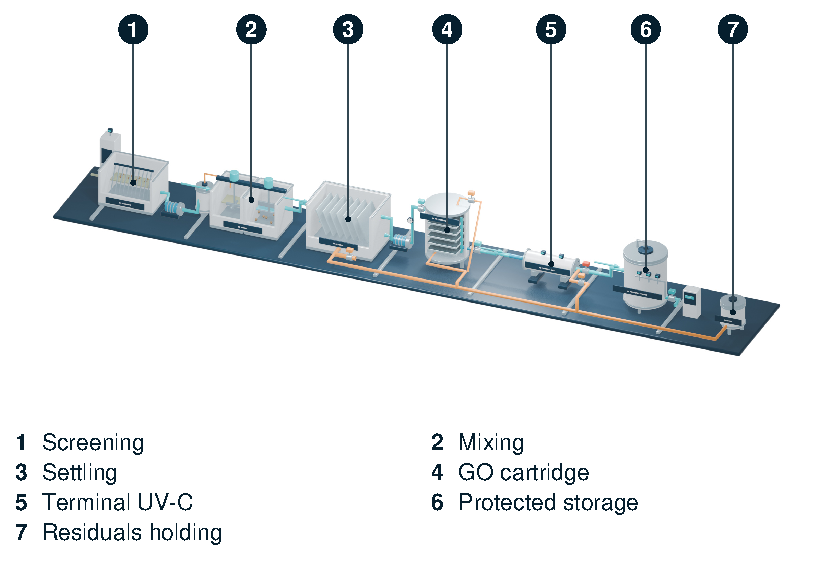
\includegraphics[width=0.60\textwidth,trim=0bp 5.5bp 0bp 5bp,clip]{figures/07_Integrated_Machine.pdf}
\caption{Integrated BLUESHIELD machine rendered in Blender. The revised series arrangement is intake, coagulation and flocculation, settling, supported GO, terminal UV-C and protected storage. Separate sludge and diverted-water routes and pressure-loop provisions address interfaces absent from a simple vessel diagram. Conceptual layout, without validated dimensions, capacity or performance.}\label{fig:machine}
\end{minipage}\par\vspace{2pt}

\par\vspace{2pt}\noindent\begin{minipage}{\linewidth}\makeatletter\def\@captype{figure}\makeatother\centering
\centering
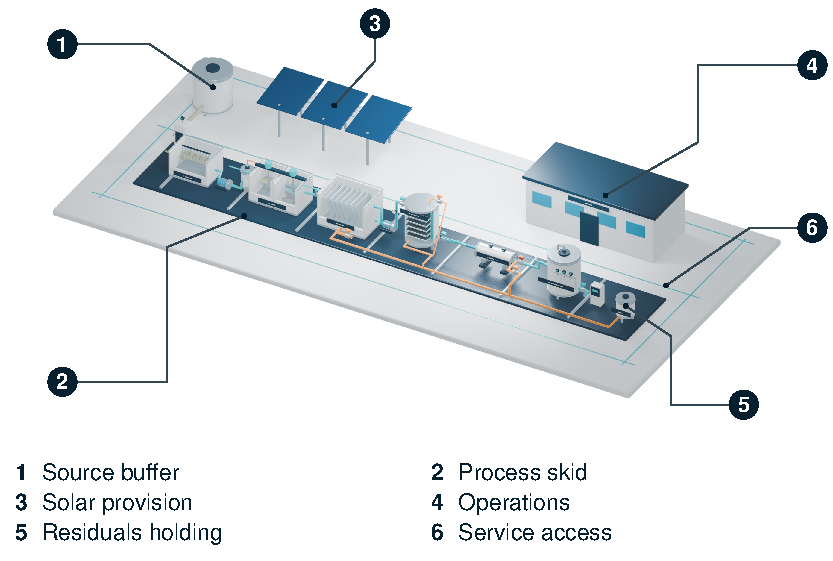
\includegraphics[width=0.60\textwidth,trim=0bp 5.5bp 0bp 2bp,clip]{figures/08_Industrial_Installation.pdf}
\caption{Revised industrial implementation rendered in Blender, developed from the earlier project setup. Treatment, residuals and service areas are spatially distinguished. This is a proposed installation arrangement, not an operating plant, structural design or demonstrated production capacity.}\label{fig:industrial}
\end{minipage}\par\vspace{2pt}
\begin{multicols}{2}


\fontsize{10}{13.42}\selectfont
\section{Conclusion}

BLUESHIELD FILTER is proposed to address the treatment and operational difficulties of obtaining usable water during floods. The study combines an exploratory stakeholder survey with component evidence to define a treatment sequence, preliminary engineering requirements and priorities for prototype development. Its contribution is to connect anticipated user and operator needs with functions that can be examined through subsequent design and testing.

The proposed sequence comprises screened intake, controlled coagulation and flocculation, settling with sludge removal, a supported graphene oxide (GO) cartridge, terminal UV-C treatment and protected storage. Screening addresses coarse debris, while coagulation, flocculation and settling prepare water for the membrane. The supported GO stage provides a candidate separation platform whose function depends on material, support and operating conditions. UV-C follows filtration as the final disinfection stage before hygienic dispensing. Physicochemical sensors, flow measurement and UV-status monitoring support supervision, maintenance and fault response; appropriate laboratory measurements remain necessary to verify water quality.

The formulation integrates these treatment interfaces with practical operating provisions. Separate sludge and diverted-water routes, sampling and cleaning access, contained membrane media, a pressure-compatible feed arrangement and a proposed interlocked outlet specify the responsibilities of individual modules. The stage and installation models communicate these relationships and identify decisions needed before fabrication. This integration provides a structured basis for comparison and modification, with each proposed function linked to an observable operating condition or prospective test.

The reported survey of 125 students and professionals found favorable perceptions of technical feasibility, anticipated effectiveness and monitoring usefulness of 84.0\%, 86.4\% and 92.0\%, respectively. In the reported 25-professional component, 20 participants identified environmental conditions, 15 identified energy efficiency or scalability, and 18 identified affordability concerns. These findings direct attention toward source-specific operation, complete-cycle energy accounting, accessible consumables and service requirements. The ratings express expectations within the recruited sample; they do not measure treatment performance or establish household adoption.

The engineering scenarios connect these priorities to measurable design choices. A 20-L batch with an assumed 90\% recoverable fraction, 81 minutes of pretreatment and 10 L/h discharge yields 18 L over 3.15 hours, approximately 5.71 L/h across the cycle. The recoverable fraction is a lumped volume allowance; filling, cleaning and operator delays are omitted, so this calculation is not a continuous production rating. At assumed fluxes of 10, 25 and 50 L\,m$^{-2}$\,h$^{-1}$, delivering 10 L/h requires 1.0, 0.4 and 0.2 m$^2$ of membrane area. Pressure and UV-exposure calculations identify measurements required to establish sizing and performance.

Recruitment procedures, the complete questionnaire, collection dates, participant responses and interview transcripts are unavailable, and the sample is concentrated in Bangladesh and selected disciplines. Conflicting impact-item summaries remain excluded from interpretation. Consent and ethics documentation have not been recovered, preventing verification of the original collection procedures. These limitations restrict reproducibility and generalizability, while absent treatment experiments leave contaminant removal, potability, operating cost and sustained performance unresolved.

Further work should combine documented survey expansion with staged prototype evaluation. Recruitment toward at least 350 participants should follow a justified sampling and study-size plan, include intended users and operators, and record regional and seasonal context. A larger count alone will not correct selection bias. Prototype testing should establish source-water envelopes through jar tests, characterize the supported GO architecture, and measure fouling, material release, permeate quality and cleaning performance. UV exposure and microbial inactivation, sensor calibration, outlet interlocks and storage hygiene require evaluation. Modifications to membrane area, pressure supply, batch scheduling, replaceable modules and power provision should follow measured throughput, energy, maintenance and cost data. Comparison with established options and observation of sustained household use would then determine where the concept offers practical benefit. BLUESHIELD presently provides a survey-informed, testable design direction for floodwater treatment.


\begin{thebibliography}{99}
\bibitem{r1} M. S. Islam et al., ``Faecal contamination of drinking water sources of Dhaka city during the 2004 flood in Bangladesh and use of disinfectants for water treatment,'' J. Appl. Microbiol., vol. 103, no. 1, pp. 80--87, 2007, doi: \href{https://doi.org/10.1111/j.1365-2672.2006.03234.x}{10.1111/j.1365-2672.2006.03234.x}.

\bibitem{r2} J. Luoto et al., ``What point-of-use water treatment products do consumers use? Evidence from a randomized controlled trial among the urban poor in Bangladesh,'' PLoS ONE, vol. 6, no. 10, Art. no. e26132, 2011, doi: \href{https://doi.org/10.1371/journal.pone.0026132}{10.1371/journal.pone.0026132}.

\bibitem{r3} A. J. Pickering et al., ``Differences in field effectiveness and adoption between a novel automated chlorination system and household manual chlorination of drinking water in Dhaka, Bangladesh: A randomized controlled trial,'' PLoS ONE, vol. 10, no. 3, Art. no. e0118397, 2015, doi: \href{https://doi.org/10.1371/journal.pone.0118397}{10.1371/journal.pone.0118397}.

\bibitem{r4} C. C. Castro-Jiménez, J. C. Saldarriaga-Molina, and E. F. García, ``Physical-chemical characterisation of an alum-based water treatment sludge in different raw water turbidity scenarios,'' Heliyon, vol. 10, no. 17, Art. no. e37579, 2024, doi: \href{https://doi.org/10.1016/j.heliyon.2024.e37579}{10.1016/j.heliyon.2024.e37579}.

\bibitem{r5} I. Krupińska, ``Aluminium drinking water treatment residuals and their toxic impact on human health,'' Molecules, vol. 25, no. 3, Art. no. 641, 2020, doi: \href{https://doi.org/10.3390/molecules25030641}{10.3390/molecules25030641}.

\bibitem{r6} C.-N. Yeh, K. Raidongia, J. Shao, Q.-H. Yang, and J. Huang, ``On the origin of the stability of graphene oxide membranes in water,'' Nat. Chem., vol. 7, no. 2, pp. 166--170, 2015, doi: \href{https://doi.org/10.1038/nchem.2145}{10.1038/nchem.2145}.

\bibitem{r7} J. Abraham et al., ``Tunable sieving of ions using graphene oxide membranes,'' Nat. Nanotechnol., vol. 12, pp. 546--550, 2017, doi: \href{https://doi.org/10.1038/nnano.2017.21}{10.1038/nnano.2017.21}.

\bibitem{r8} L. Qian et al., ``Amino acid cross-linked graphene oxide membranes for metal ions permeation, insertion and antibacterial properties,'' Membranes, vol. 10, no. 10, Art. no. 296, 2020, doi: \href{https://doi.org/10.3390/membranes10100296}{10.3390/membranes10100296}.

\bibitem{r9} H. Liu, X. Huang, Y. Wang, B. Kuang, and W. Li, ``Nanowire-assisted electrochemical perforation of graphene oxide nanosheets for molecular separation,'' Nat. Commun., vol. 15, Art. no. 164, 2024, doi: \href{https://doi.org/10.1038/s41467-023-44626-9}{10.1038/s41467-023-44626-9}.

\bibitem{r10} K. Oguma, R. Kita, H. Sakai, M. Murakami, and S. Takizawa, ``Application of UV light emitting diodes to batch and flow-through water disinfection systems,'' Desalination, vol. 328, pp. 24--30, 2013, doi: \href{https://doi.org/10.1016/j.desal.2013.08.014}{10.1016/j.desal.2013.08.014}.

\bibitem{r11} C. Farrell, F. Hassard, B. Jefferson, T. Leziart, A. Nocker, and P. Jarvis, ``Turbidity composition and the relationship with microbial attachment and UV inactivation efficacy,'' Sci. Total Environ., vol. 624, pp. 638--647, 2018, doi: \href{https://doi.org/10.1016/j.scitotenv.2017.12.173}{10.1016/j.scitotenv.2017.12.173}.

\bibitem{r12} P. Jarvis, O. Autin, E. H. Goslan, and F. Hassard, ``Application of ultraviolet light-emitting diodes (UV-LED) to full-scale drinking-water disinfection,'' Water, vol. 11, no. 9, Art. no. 1894, 2019, doi: \href{https://doi.org/10.3390/w11091894}{10.3390/w11091894}.

\bibitem{r13} D. Gillett and A. Marchiori, ``A low-cost continuous turbidity monitor,'' Sensors, vol. 19, no. 14, Art. no. 3039, 2019, doi: \href{https://doi.org/10.3390/s19143039}{10.3390/s19143039}.

\bibitem{r14} R. Bogdan, C. Paliuc, M. Crisan-Vida, S. Nimara, and D. Barmayoun, ``Low-cost Internet-of-Things water-quality monitoring system for rural areas,'' Sensors, vol. 23, no. 8, Art. no. 3919, 2023, doi: \href{https://doi.org/10.3390/s23083919}{10.3390/s23083919}.

\bibitem{r15} E. von Elm, D. G. Altman, M. Egger, S. J. Pocock, P. C. Gøtzsche, and J. P. Vandenbroucke, ``The Strengthening the Reporting of Observational Studies in Epidemiology (STROBE) statement: Guidelines for reporting observational studies,'' PLoS Med., vol. 4, no. 10, Art. no. e296, 2007, doi: \href{https://doi.org/10.1371/journal.pmed.0040296}{10.1371/journal.pmed.0040296}.

\bibitem{r16} A. Tong, P. Sainsbury, and J. Craig, ``Consolidated criteria for reporting qualitative research (COREQ): A 32-item checklist for interviews and focus groups,'' Int. J. Qual. Health Care, vol. 19, no. 6, pp. 349--357, 2007, doi: \href{https://doi.org/10.1093/intqhc/mzm042}{10.1093/intqhc/mzm042}.

\bibitem{r17} C. Han et al., ``Quasi-vertically asymmetric channels of graphene oxide membrane for ultrafast ion sieving,'' Nat. Commun., vol. 16, Art. no. 1020, 2025, doi: \href{https://doi.org/10.1038/s41467-025-56358-z}{10.1038/s41467-025-56358-z}.

\bibitem{epa_turbidity2004} U.S. Environmental Protection Agency, \emph{Long Term 1 Enhanced Surface Water Treatment Rule: Turbidity Provisions Technical Guidance Manual}, EPA 816-R-04-007, Aug. 2004. [Online]. Available: \url{https://nepis.epa.gov/Exe/ZyPURL.cgi?Dockey=30005ZHV.TXT}

\bibitem{epa_nutrient2010} U.S. Environmental Protection Agency, \emph{Nutrient Control Design Manual}, EPA/600/R-10/100, Aug. 2010, sec. 9.6.2.1. [Online]. Available: \url{https://nepis.epa.gov/Exe/ZyPURL.cgi?Dockey=P1008KTD.TXT}

\bibitem{epa_uv2006} U.S. Environmental Protection Agency, \emph{Ultraviolet Disinfection Guidance Manual for the Final Long Term 2 Enhanced Surface Water Treatment Rule}, EPA 815-R-06-007, Nov. 2006. [Online]. Available: \url{https://www.epa.gov/system/files/documents/2022-10/ultraviolet-disinfection-guidance-manual-2006.pdf}

\bibitem{doe_pump2005} U.S. Department of Energy, ``Test for pumping system efficiency,'' \emph{Energy Tips---Pumping Systems}, Tip Sheet 4, Sep. 2005. [Online]. Available: \url{https://www1.eere.energy.gov/manufacturing/tech_assistance/pdfs/test_pumping_system__pumping_systemts4.pdf}

\bibitem{who_hwt2018} World Health Organization, \emph{WHO International Scheme to Evaluate Household Water Treatment Technologies: Harmonized Testing Protocol---Technology Non-Specific}, ver. 2.1, Geneva, Switzerland, Aug. 2018. [Online]. Available: \url{https://www.who.int/docs/default-source/wash-documents/water-safety-and-quality/household-water-treatment/hwt-scheme-harmonized-test-protocol-2018.pdf}

\bibitem{r18} L. M. T. Broyles, E. L. Pakhtigian, S. Aziz, A. S. Akanda, and A. Mejia, ``Seasonal variation in household water insecurity in rural Bangladesh: A longitudinal analysis,'' PLOS Water, vol. 2, no. 7, Art. no. e0000157, 2023, doi: \href{https://doi.org/10.1371/journal.pwat.0000157}{10.1371/journal.pwat.0000157}.
\end{thebibliography}

\end{multicols}
\end{document}
